\documentclass[12pt]{pom_thesis}
\usepackage[table]{xcolor}
\usepackage[]{algorithm2e}
\usepackage{tikz}
\usepackage{ifthen}
\usepackage{listings}
\usepackage{color}

\definecolor{dkgreen}{rgb}{0,0.6,0}
\definecolor{gray}{rgb}{0.5,0.5,0.5}
\definecolor{mauve}{rgb}{0.58,0,0.82}

\lstset{frame=tb,
	language=Python,
	aboveskip=3mm,
	belowskip=3mm,
	showstringspaces=false,
	columns=flexible,
	basicstyle={\small\ttfamily},
	numbers=none,
	numberstyle=\tiny\color{gray},
	keywordstyle=\color{blue},
	commentstyle=\color{dkgreen},
	stringstyle=\color{mauve},
	breaklines=true,
	breakatwhitespace=true,
	tabsize=3
}
% This first part of the file is called the PREAMBLE. It includes
% customizations and command definitions. The preamble is everything
% between \documentclass and \begin{document}.
\usepackage{amsthm}
\newtheorem{theorem}{Theorem}
\usepackage[margin=1in]{geometry}  % set the margins to 1in on all sides
\usepackage{graphicx}              % to include figures
\usepackage{amsmath}               % great math stuff
\usepackage{amsfonts}              % for blackboard bold, etc
\usepackage{amsthm}                % better theorem environments
\usepackage{changepage}
\usepackage{lipsum}                     % Dummytext
\usepackage{xargs}                      % Use more than one optional parameter in a new commands
 % Coloured text etc.
% 
\usepackage[colorinlistoftodos,prependcaption,textsize=tiny]{todonotes}
\newcommandx{\unsure}[2][1=]{\todo[linecolor=red,backgroundcolor=red!25,bordercolor=red,#1]{#2}}
\newcommandx{\change}[2][1=]{\todo[linecolor=blue,backgroundcolor=blue!25,bordercolor=blue,#1]{#2}}
\newcommandx{\info}[2][1=]{\todo[linecolor=OliveGreen,backgroundcolor=OliveGreen!25,bordercolor=OliveGreen,#1]{#2}}
\newcommandx{\improvement}[2][1=]{\todo[linecolor=Plum,backgroundcolor=Plum!25,bordercolor=Plum,#1]{#2}}
\newcommandx{\thiswillnotshow}[2][1=]{\todo[disable,#1]{#2}}
\newcommand{\blockmatrix}[9]{
	\draw[draw=#4,fill=#5] (0,0) rectangle( #1,#2);
	\ifthenelse{\equal{#6}{true}}
	{
		\draw[draw=#7,fill=#8] (0,#2) -- (#9,#2) -- ( #1,#9) -- ( #1,0) -- ( #1 - #9,0) -- (0,#2 -#9) -- cycle;
	}
	{}
	\draw ( #1/2, #2/2) node { #3};
}

% Quick implementation of a tikz right parenthesis
% \rightparen{width}
\newcommand{\rightparen}[1]{
	\begin{tikzpicture} 
	\draw (0,#1/2) arc (0:30:#1);
	\draw (0,#1/2) arc (0:-30:#1);
	\end{tikzpicture}%this comment is necessary
}

% Quick implementation of a tikz left parenthesis
% \leftparen{width}
\newcommand{\leftparen}[1]{
	\begin{tikzpicture} 
	\draw (0,#1/2) arc (180:150:#1);
	\draw (0,#1/2) arc (180:210:#1);
	\end{tikzpicture}%this comment is necessary
}

% Unframed block matrix, "m" prefix to match fbox, mbox
% \blockmatrix[r,g,b]{width}{height}{text}
\newcommand{\mblockmatrix}[4][none]{
	\begin{tikzpicture} 
	\ifthenelse{\equal{#1}{none}}
	{
		\blockmatrix{#2}{#3}{#4}{none}{none}{false}{none}{none}{0.0}
	}
	{
		\definecolor{fillcolor}{rgb}{#1}
		\blockmatrix{#2}{#3}{#4}{none}{fillcolor}{false}{none}{none}{0.0}
	}
	\end{tikzpicture}%this comment is necessary
}

% Framed block matrix
% \fblockmatrix[r,g,b]{width}{height}{text}
\newcommand{\fblockmatrix}[4][none]{
	\begin{tikzpicture} 
	\ifthenelse{\equal{#1}{none}}
	{
		\blockmatrix{#2}{#3}{#4}{black}{none}{false}{none}{none}{0.0}
	}
	{
		\definecolor{fillcolor}{rgb}{#1}
		\blockmatrix{#2}{#3}{#4}{black}{fillcolor}{false}{none}{none}{0.0}
	}
	\end{tikzpicture}%this comment is necessary
}

% Diagonal block matrix
% \dblockmatrix[r,g,b]{width}{height}{text}
\newcommand{\dblockmatrix}[4][none]{
	\begin{tikzpicture} 
	\ifthenelse{\equal{#1}{none}}
	{
		\blockmatrix{#2}{#3}{#4}{black}{none}{true}{black}{none}{0.35cm}
	}
	{
		\definecolor{fillcolor}{rgb}{#1}
		\blockmatrix{#2}{#3}{#4}{black}{none}{true}{black}{fillcolor}{0.35cm}
	}
	\end{tikzpicture}%this comment is necessary
}


% Diagonal block matrix, but exposes diagonal offset
% \diagonalblockmatrix[r,g,b]{width}{height}{text}
\newcommand{\diagonalblockmatrix}[5][none]{
	\begin{tikzpicture} 
	
	\ifthenelse{\equal{#1}{none}}
	{
		\blockmatrix{#2}{#3}{#4}{black}{none}{true}{black}{none}{#5}
	}
	{
		\definecolor{fillcolor}{rgb}{#1}
		\blockmatrix{#2}{#3}{#4}{black}{none}{true}{black}{fillcolor}{#5}
	}
	
	\end{tikzpicture}%necessary comment
}

\newcommand{\valignbox}[1]{
	\vtop{\null\hbox{#1}}% necessary comment
}

% a hack so that I don't have to worry about the number of columns or
% spaces between columns in the tabular environment
\newenvironment{blockmatrixtabular}
{% necessary comment
	\begin{tabular}{
			@{}l@{}l@{}l@{}l@{}l@{}l@{}l@{}l@{}l@{}l@{}l@{}l@{}l@{}l@{}l@{}l@{}l@{}l@{}l
			@{}l@{}l@{}l@{}l@{}l@{}l@{}l@{}l@{}l@{}l@{}l@{}l@{}l@{}l@{}l@{}l@{}l@{}l@{}l
			@{}l@{}l@{}l@{}l@{}l@{}l@{}l@{}l@{}l@{}l@{}l@{}l@{}l@{}l@{}l@{}l@{}l@{}l@{}l
			@{}
		}
	}
	{
	\end{tabular}%necessary comment
}
% various theorems, numbered by section


\DeclareMathOperator{\id}{id}

\newcommand{\bd}[1]{\mathbf{#1}}  % for bolding symbols
\newcommand{\RR}{\mathbb{R}}      % for Real numbers
\newcommand{\ZZ}{\mathbb{Z}}      % for Integers
\newcommand{\col}[1]{\left[\begin{matrix} #1 \end{matrix} \right]}
\newcommand{\comb}[2]{\binom{#1^2 + #2^2}{#1+#2}}
\usepackage{graphicx}
\usepackage{csquotes}
\usepackage{lipsum}
\newcommand\tab[1][1cm]{\hspace*{#1}}

\begin{document}


\nocite{*}

\title{Data Representation as Low Rank Matrix Factorization}


\author{Ziv Epstein \\ 
	\texttt{ziv.epstein@pomona.edu}}
\advisor{Blake Hunter}
\maketitle
\pagenumbering{arabic}
\tableofcontents
\newpage


\abstract{ 
	Non-negative matrix factorization (NNMF) is a powerful representational model to detect underlying structure from noisy data. In this thesis, I explore a suite of NNMF algorithms, and connect them to the cognitive science literature, which is also concerned about detecting underlying from noisy data (think visual perception).
	In this vein, I introduce the notion of hierarchical manifold NNMF as an NNMF analogy that echoes many of the important functionality of the human visual perception system.
	\begin{center}
	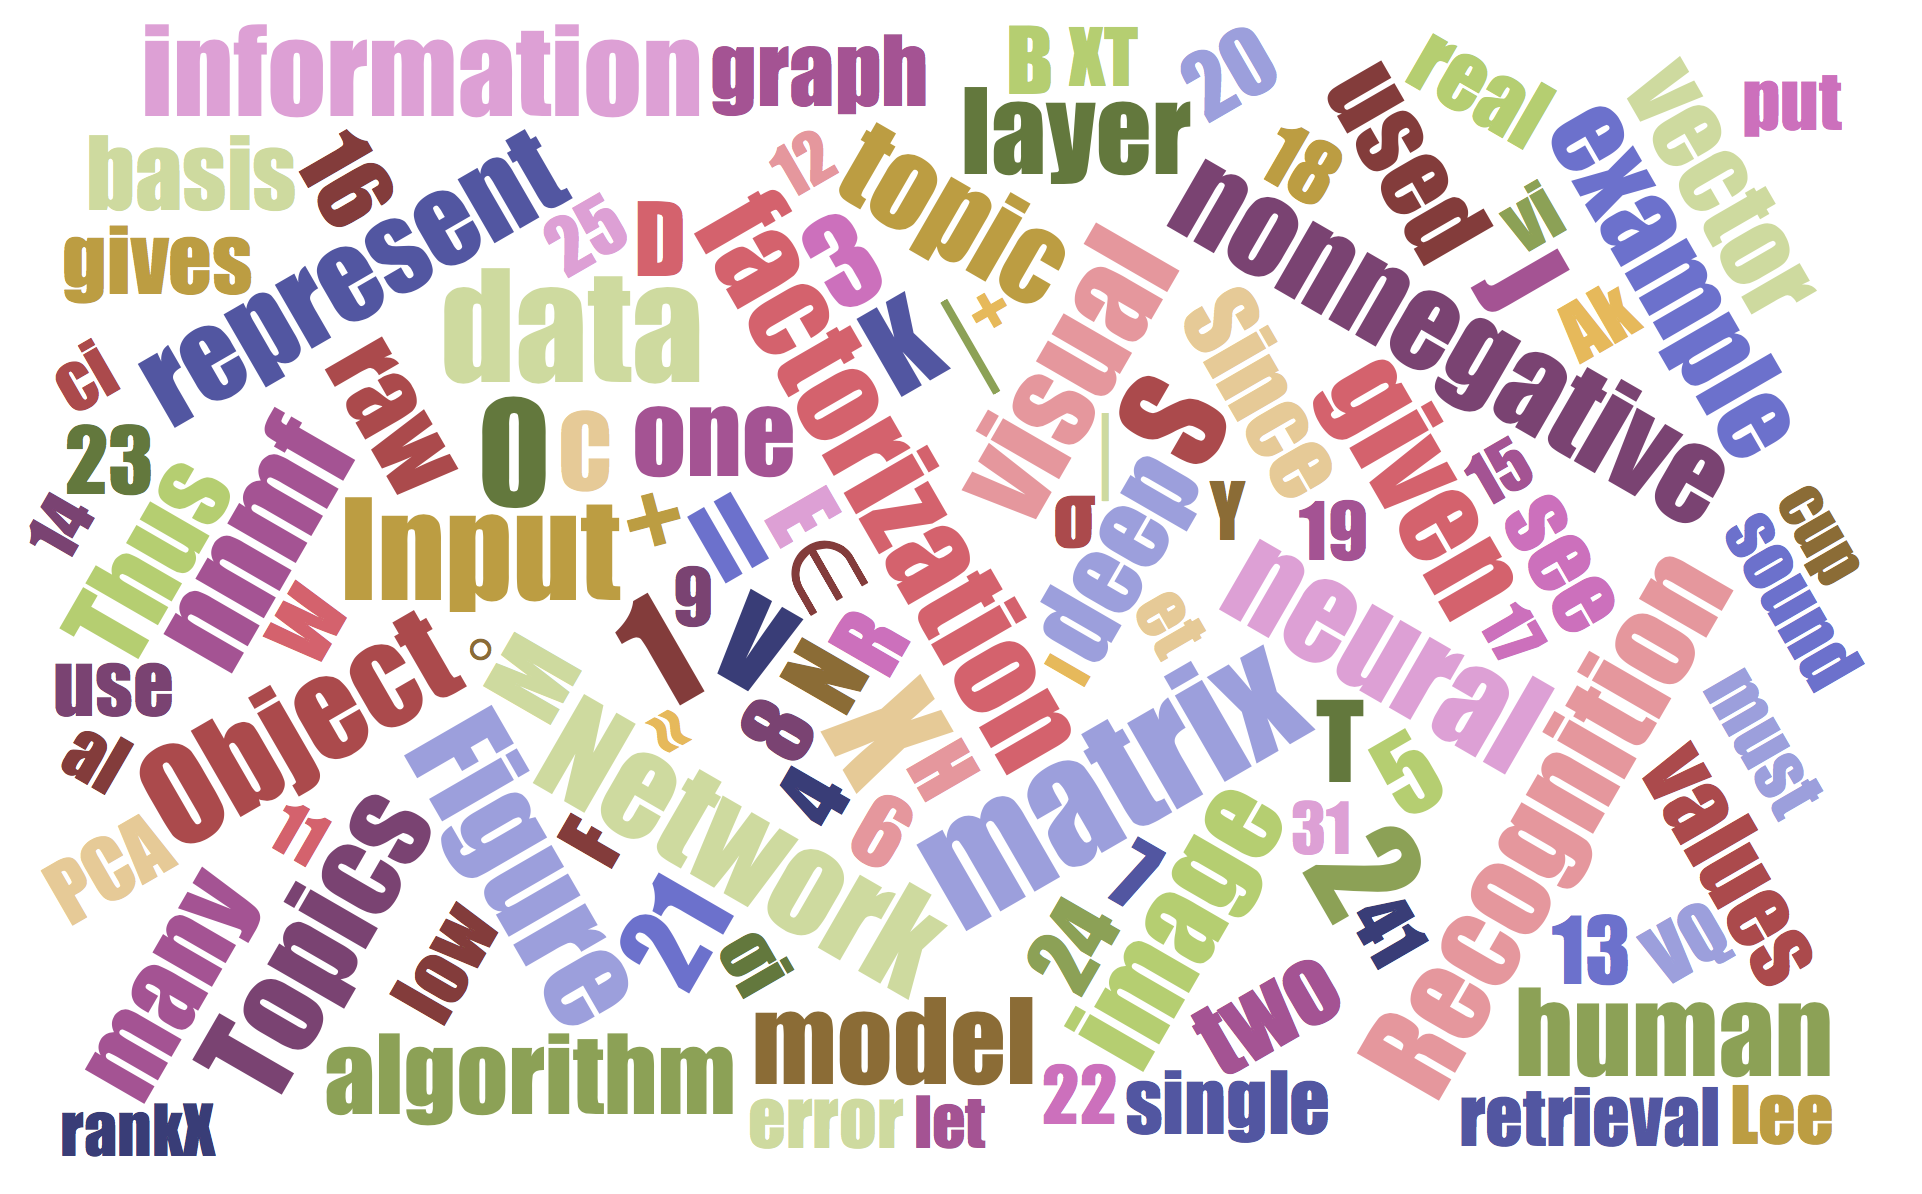
\includegraphics[width=18cm]{wordcloud}
\end{center}
	}
	\newpage
\section*{Foreword}
This thesis began as an exploration of the suite of algorithms that constitute non-negative matrix factorization (NNMF). Indeed because it learns robust topics in text and has strong intuitions in linear algebra, NNMF is a very a fascinating domain suitable for further inquiry. 

Parallel to these studies, I became very interested with another facet of NNMF. In reading many of the foundational papers in the field, such as Ngoc-Diep Ho's PhD Dissertation at Ecole Polytechnique \cite{ho2008nonnegative} and Lee and Seung's 1999 Nature paper \cite{lee1999learning}, I noticed a pattern. The papers would always begin with several sentences relating the work to human cognition. For example, Lee and Sueng begin their seminal work by saying that ``there
is psychological and physiological evidence for parts-based representations in the brain, and certain computational theories of object recognition rely on such representations. But little is known about how brains or computers might learn the parts of objects.'' They then proceed to dive into a technical overview of the algorithms they proposed \cite{lee1999learning}. This topic sentence connecting to human cognition is always short, broad but \textit{present}.

To my knowledge, a meditation on the connections between NNMF and the cognitive underpinnings of human understanding that exceeds a couple sentences does not exist. This is of course partially because such ideas have been channeled into discourse relating human understanding and more general and plastic forms of machine learning, such as neural networks. But the structured nature of NNMF provides interesting comparisons with the human visual system. 
In this thesis, I both explore the algorithms and mine the cognitive science literature in an attempt to build a unifying theory. While the success of this pursuit is questionable, I do think it is an interesting attempt to blend these two ideas in an engaging and creative way.
\begin{chapter}{Introduction}
	There is a growing interest in the computational and mathematical sciences in the development of algorithms that can automatically create understanding of data pertaining to some phenomenon. As an explosion of data collection and distribution systems have become the mainstream, there is now more data available than humans observers to understand it. Thus the need for automated algorithms that can infer patterns and relationships within data is self evident. 
	
	Here, I will consider the case were data is represented as a well-structured and  real-valued matrix. This approach can represent data from a large range of domains, such as sound, natural language, visual images and networks. Thus, many of the algorithms and heuristics I explore here are domain general, and can be applied with success to a range of settings. 
	
	My particular focus in this thesis is the notion of \textit{low-dimensional representations of data}. A real valued matrix $X$ that represents a collection of sounds, natural language documents, images or networks taken from real world settings will necessarily be noisy and not optimally structured. One canonical challenge (that we will dub ``The Representation Problem'') is to find a $X' \approx X$ that well approximates the original data's structure, but with $\operatorname{rank}(X') << \operatorname{rank}(X)$. A low rank approximation of the data gives a sparse representation that captures the underlying latent structure of the data. 
	
	This approach also has explanatory power. Let $r = \operatorname{rank}(X')$ and $b= (b_1,b_2,\cdots,b_r)$ be a basis for the columns of $X'$. Depending on the constraints imposed on the $b_i$'s, they can have many different interpretations. For example, when the $b_i$'s are constrained to be orthonormal, the resulting algorithm is Principal Component Analysis (PCA), which ``supplies the user with a lower-dimensional projection of the object when viewed from its most informative viewpoint.'' \cite{jolliffe2002principal}
	
	Since our mission is to emulate human understanding, a natural starting place for inspiration is the human brain itself. Indeed there is a long-standing tradition in computer and information science to algorithmically model the information processing systems the brain uses to make sense of the world. However, I hope to also go one step deeper. In addition to an overview of many of the important algorithms used today, we will explore the cognitive implications of these algorithms. In particular, I aim to invert the paradigm of using neural architecture to inform algorithms: I will use algorithms to inform notions of neural architecture. By creating a bilateral dialogue between the cognitive and computer sciences, I hope this work will help to bridge the gaps between the two fields by I) equipping the cognitive ideas of neural information processing with a notational formalism consist with the algorithms research and II) contextualizing the algorithms research whereby it is clear how it might relate to the acquisition of human knowledge.
	
	
	The overarching organization structure of this thesis is to first begin with the large, cognitive notions I will be exploring, then I will accumulate the complexity of nonnegative matrix factorization algorithms to arrive at a final correspondence between the theory and application. Chapter 2 begins with an overview of several theories used to understand the human visual processing machine. Chapter 3 introduces several canonical algorithms for representing data, including NNMF, which is the algorithm I will focus on in the thesis. Chapter 4 explores four different types of data that can be represented as a real-valued matrix, and gives some intuition as to what the results of NNMF look like in that domain. Chapter 5 introduces the notion of supervised learning into the NNMF objective function, and argues the importance of manifold learning in simulating the human visual processing system. Chapter 6 builds on the functionality of NNMF by adding a hierarchical component to the model, and then subsequently expands this notion of hierarchy by generalizing to deep, recursive models. 
\end{chapter}

\begin{chapter}{Theories for Human Image Understanding}
	The general class of algorithms I consider have in the common the fact that they take as input a large amount of noisy, somewhat structured data, and output some unified high-level notion of underlying pattern. 
	\begin{figure}[h]
		\label{cup}
		\centering
		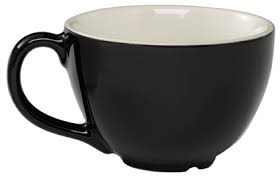
\includegraphics[width=3in]{cup}
		\caption{How does your brain take the raw retinal activations of this picture and produce a mental representation of a cup?}
	\end{figure}
	Thus in many ways they emulate the most successful machine that converts raw data to high-level concepts: the human visual system. When observing at a cup, our brains take  in thousands of raw retinal activities, and through a complex schema of neural information processing systems, result in a high-level conceptualization of a cup. The intricacies of this pipeline are not fully understood, but many of the driving mechanisms are. To motivate the algorithmic approach, I begin with a short overview of the pervading theories for human image understanding. 

\section{Part-based recognition and visual perception}
A given object can project an uncountable infinitude of possible visual configurations to the human retina. Thus the phenomenon of how raw visual input to the visual system is represented as robust concepts in the human mind has long haunted philosophers, cognitive scientists, mathematicians and computer scientists. Empirical observation imposes several axioms that any repsectable theory of object recognition must take into account, which Biederman enumerates \cite{biederman1987recognition}:
\begin{enumerate}
	\item \textbf{Imprecise attention to detail:} ``Access to the mental representation of an object should not be dependent on the absolute judgments of quantitative detail. For example, distinguishing among just several levels of the degree of curvature or length of an object typically requires more time that that retuqired for the identifcation of the object itself.''
	\item \textbf{Topological fuzziness:} ``The information that is the basis for recognition should be relatively invariant with respect to orientation and modest degradation'.'
	\item \textbf{Plasticity:} ``Partial matches should be computable. A theory of object interpretation should have some principled means for computing a match for occluded, partial or new exemplars of a given category.''
\end{enumerate}
These axioms are central to task of modeling, and will be used by the cognitive and mathematical models put forward here. A large number of explanatory theories have been proposed over the years for this phenomenon of object recognition. One extremal idea is the structuralist position which posits that ``the perception of whole figures is nothing more than the concatenation of primitive perceptual elements.'' \cite{palmer1977hierarchical}. Another extremal approach, born out of Gestalt theory, claims that the recognition of complex objects is an indivisible process, which cannot be reconstructed by considering the nature and properties of its constituent parts.  The most performant theories lie within the simplex defined by these holistic and atomic extrema. One such theory, the Recognition-by-Components (RBC) theory proposed by Biederman proposes a sparse vocabulary of atoms and a schema for how these components can be conglomerated to represent in memory (see Figure~\ref{fig: rbc}) \cite{biederman1987recognition}.
\begin{figure}
	\label{fig: rbc}
	\centering
	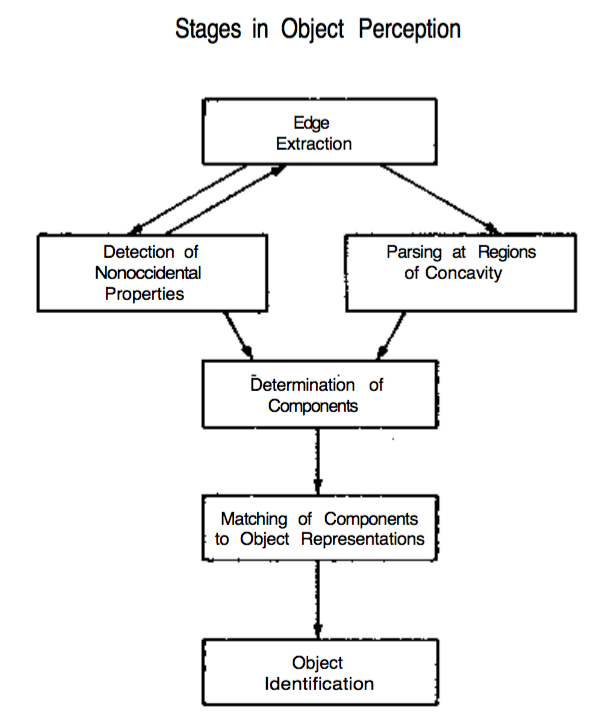
\includegraphics[width=6cm]{rbc}
	\caption{Processing stages for object recognition proposed by the RBC Theory. Adapted from \cite{biederman1987recognition}}
\end{figure}
First, edges are extracted from the raw sensory data received from the optical system. Local properties of the input, such as luminance, texture and color, aid in providing robust edge segmentations. Then, in parallel, the parsing of the concave regions and the identification of nonaccidental properties is performed. The latter provides ``critical constraints on the identity of the components. Then these processes coalesce to form a specific arrangement of components, which are then matched against pre-existing representations in memory. The representation that best ``matches'' the observed arrangement gives rise to the actual object identification. 

Since RBC uniquely relates to the visual system, the components Biederman proposes are a set of generalized cones called \textbf{geons} (for ``geometric ions'') \cite{biederman1987recognition}.
A victory for RBC is its explanatory vastness with a small number of components. Biederman suggests that 36 geons is sufficient to represent all objects that humans can differentiate between. 

RBC has two heuristics that we will primary draw upon for formalizing this theory of object recognition with formal models. The first is this ability to represent the nuance of human perception with a small number of components. In mathematical terms, these components form a linearly independent \textbf{basis}, by which any object, $O$, can be approximated:
\begin{equation} \label{eq:1}O = \sum_{i=1}^d \alpha_i b_i\end{equation}
where $d$ is much smaller than the space of possible objects. Natural questions that arise from this model of human perception are 1) What is sufficient for $d$? Biederman proposes $d=36$ is sufficient of visual object recognition, but what about other domains? and 2) How are these bases, $b_i$ learned? Biederman suggests that $b_i$ is a volumetric cone, but gives no explanation for how this components emerge from the human visual system. 

The second heuristic of RBC we will use the schematic for recognition (see Figure \ref{fig: rbc}). This schema gives us a roadmap for a suite of algorithms we will use to generate representational models (see Section \ref{chapter:techniques}). 
\section{Knowledge representation as information retrieval}
The RBC Theory puts forward a highly structured representation of a given input $O$ as described in Equation \ref{eq:1}. It then suggests that this representation is then procedurally matched with a preexisting notion in memory towards recognition. To understand how this matching occurs, we turn to Minsky's framework for representing knowledge \cite{minsky1975framework}. Minsky thinks of memory as a collection of \textbf{frames}, which is a data structure that represents a stereotyped situation, space or object \cite{minsky1975framework}. In particular, a frame is a hierarchical network of nodes and relations which correspond to that which the frame represents. In particular, the ``top levels'' of the network are fixed. They represent entities and relations that are always true about the frame's content. The lower lever has \textbf{terminals}, empty ``slots'' to be filled with raw input or data. These terminals carry with them a set of rules (which are frames themselves) which specify the necessary conditions for assignment that terminal. 

Large collections of these frames are aggregated into structures called \textbf{frame-systems}, where related frames are proximal. In particular, actions in the world correspond to \textbf{transformations} in the frame-system, whereby similar objects have a smooth transformation between them. For example, different frames might correspond to observing a room at different angles, and the transformation between adjacent frames corresponds to the observer moving to change their vantage point \cite{minsky1975framework}. These frame-systems are further connected into a \textbf{information retrieval network}. 

After the raw sensory input of a stimulus percolates through the RBC processing system outlined in Figure 2, it finally reaches a component representation that must be matched with a frame. This process is done as follows: for a given frame $F^i$ with top levels $f^i$ and terminals $t^i$, the features of the representation are assigned to the frame's terminals, $t_i$. In the assignment sufficiently conforms for the specifications of the terminals (i.e. their corresponding frames $F_{t_i}$, and the top level nodes $f_i$), the object is identified as in the last stage of Figure 2.1. However if the proposed frame cannot conform to the terminal specifications, then the information retrieval system repeatedly puts forward another frame until a candidate fits the condition.

This process of selecting an optimal frame for representation is parallel to the optimization component of the algorithms we will discuss.  
\section{The hierarchical structure of perception}
Biederman puts forward an atomic unit of visual perception \cite{biederman1987recognition}, and Minksy extends that notion with a generalized framework for representing these atomic units \cite{minsky1975framework}. However neither of these formulations describe explicitly how raw sensory data can be accumulated into something as sophisticated as the high-level recognition of an object. Palmer puts forward a structural schematic for hierarchical perceptual representation involving structural units, values on global properties and structural relationships (see Figure \ref{fig:palmer}) \cite{palmer1977hierarchical}. 
\begin{figure}[h]
	\label{fig:palmer}
	\centering
	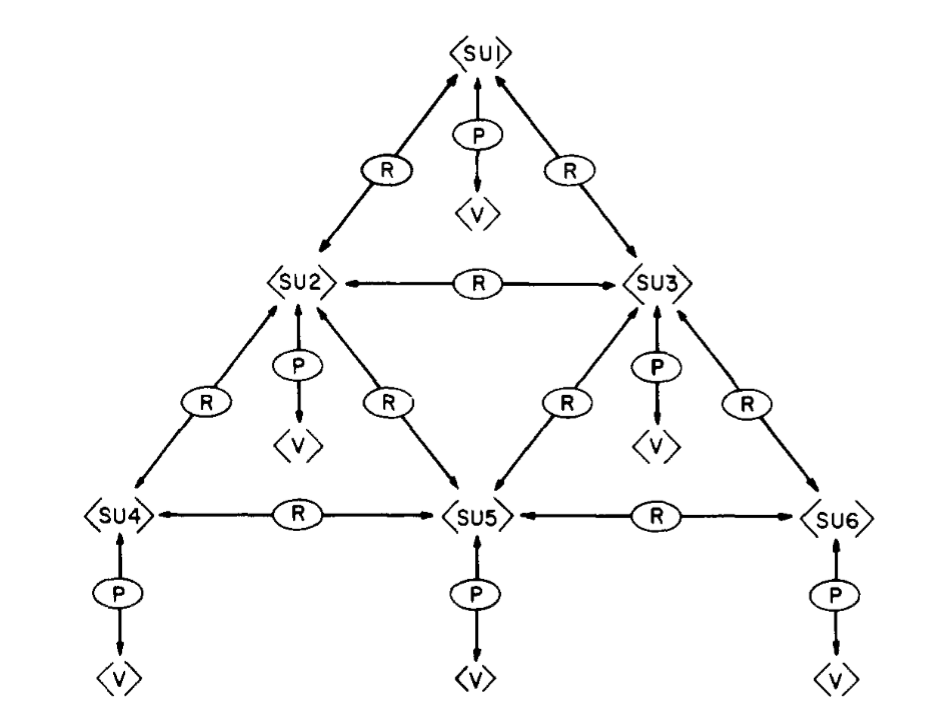
\includegraphics[width=10cm]{palmer_tree}
	\caption{The hierarchical relationship network used to represent perceptual information. At each level of the hierarchy, a structural unit (SU) is a combination of values (V) on global properties (P) and structural relationships to other structural units.  Adapted from \cite{palmer1977hierarchical}}
\end{figure}
The values of the global properties at each node of the network are a real-valued vector ``along perceptual dimensions relative to some referent.'' \cite{palmer1977hierarchical}. During the process of pattern recognition, these numeric values are used to evaluate the goodness-of-fit between some raw sensory input (that is to be identified) and some pre-existing information encoded in the network. The task of matching the sensory input to the encoded information is analogous to Minsk'y frame retrieval discussed above \cite{minsky1975framework}.
\section{Algorithmically formalizing cognitive mechanism}
\label{interp}
There are several notions of these cognitive theories put forward above that I will focus on in this thesis. In particular, I will take several of these notions from the visual perception literature, formalize them with mathematical language, and then relate them to the algorithmic formulation of NNMF.

\subsection*{Object Classification as Supervised Manifold Learning}
\label{manifold}

As we have seen, the hierarchies proposed above aim to match high-order labels to a series of raw retinal activations. For example, let $(r_1,r_2,\cdots, r_n)$ be the retinal activation of observing Figure \ref{cup}. Previous to observing the image, there exists somewhere in the perceptual hierarchy of your brain the label of cup $\ell_i$. Thus the task of object classification  can be formulated as the supervised learning of a manifold $f$, whereby $f(r_1,r_2,\cdots,r_n) = \ell_i$. We discuss this formalism and its implications further in Chaper \ref{supervised}.

\subsection*{Geons as Topics}
Biederman claims there exist a small number $d$ of atomic units that can be combined in various ways to represent complex visual stimuli \cite{biederman1987recognition}. This notion is formalied by Equation \ref{eq:1}, which claims an object $O$ is simply a linear combination of these $d$ geons. In the context of matricial algebra, we can formalize this even further as an embedding in $\mathbb{R}^m$. Figure \ref{fig:geonLC} shows a toy example for how a given complex visual simulus can be represented as a linear combination of  a small number of these atomic units. 


\begin{figure}[h]
	\label{fig:geonLC}
	\centering
	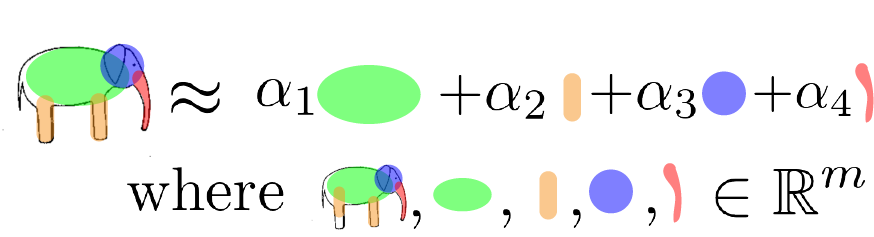
\includegraphics[width=15cm]{geonLC}
	\caption{An image can be represented as a linear combination of geons. Elephant adapted from \cite{biederman1987recognition}.}
\end{figure}
 In the context of visual perception, one might think a the natural choice is $m=3$, which corresponds to the 3-dimensional reality our retinal systems pull data from. However, it is clear that detail of an object such as elephant can't really be captured by three real numbers. So for these purposes we will assume $m$ is very large.  In the context of our example, $m$ would be the number of free parameters necessary to specify each of the four geons.  


\subsection*{Hierarchical Organization of Topics}
Many of the theories discussed above rely on a hierarchical structure of information. Indeed as can be see from Figure \ref{fig:geonLC}, the geon vectors have some relation to each other that the scalars $\alpha_i$ are designed to capture. However in concatenating all the units into an elephant, these scalar coefficients must be very specifically defined. It is clear that $\alpha_i \in \mathbb{R}$ does not give information  to reconstruct the elephant in Figure \ref{fig:geonLC}, because there are multiple dimensions of variations on which the geons are agglomerated. In addition, since both the elephant and the perspective from which one is viewing it can change,  the scalars do not only take into account spatial (x/y/z) information, but also semantic information similar to that proposed in Figure \ref{fig:palmer}. So, a information processing system sophisticated enough to perform visual perception unconstrained by movement or perspective is hierarchically organized. So a more robust characterization of the elephant in Figure \ref{fig:geonLC} would actually be a tree, as shown in Figure 2.5.
\begin{figure}[h]
\label{tree}
	\centering
	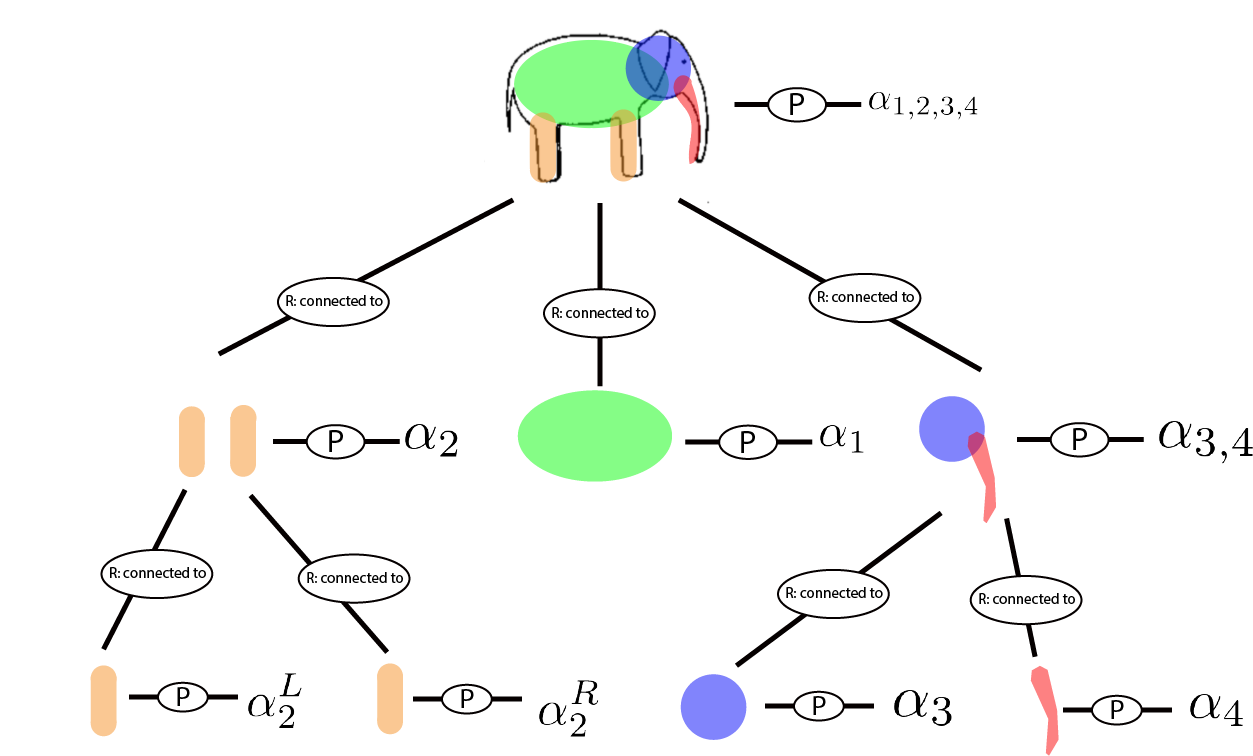
\includegraphics[width=15cm]{geonLCTree}
	\caption{The elephant from Figure \ref{fig:geonLC} is better represented as a tree of topics.}
\end{figure}
\end{chapter}


\begin{chapter}{Algorithms for Representing Data}
	\label{chapter:techniques}
\section{Singular Value Decomposition}
\label{section:svd}
The first technique to represent a matrix $X$ is to factorize it using singular value decomposition. 

\begin{theorem}
	Suppose  $X \in \mathbb{R}^{m \times n}$, then there exists a factorization, called the singular value decomposition of $X$, of the form 
	$$X= U \Sigma V^T$$ 
	where $U \in \mathbb{R}^{m \times m}$ is unitary, $\Sigma \in \mathbb{R}^{m \times n}$ with non-negative real numbers on the diagonal and $V^T \in \mathbb{R}^{n \times n}$ is unitary. 
\end{theorem}
The diagonal entries $\sigma_i$ of $\Sigma$ are called the \textbf{singular values} of $X$.

\begin{proof}(Bast) Observe that $X^TX \in \mathbb{R}^{n \times n}$ is symmetric. Thus, there exist $n$ eigenvectors $v_1,\cdots,v_r$ with corresponding eigenvalues $\lambda_1,\cdots,\lambda_r$ that are pairwise orthogonal (i.e. $v^T_iv_j=0 \ \forall i \neq j$) with $r = \text{rank}(X^TX) = \text{rank}(X)$. Furthermore, we have that $X^TX = VDV^T$, where $V=[v_1,\cdots,v_n] \in \mathbb{R}^{n\times n}$ and  $$d = \begin{bmatrix}
	\lambda_1  & 0     & \cdots             & 0    \\
	0  & \lambda_2 & \cdots & 0        \\
	\vdots  & \vdots & \ddots & \vdots &     \\
	0 & 0 & \cdots & \lambda_n
	\end{bmatrix}.$$ 
	Since $v_i$ is an eigenvector for $X^TX$, observe that $XX^TXv_i = X\lambda_iv_i=\lambda_iXv_i$. Which is to say that if  $v_i$ is an eigenvector for $X^TX$, then  $Xv_i$ is an eigenvector for $XX^T$ with the same eigenvalue $\lambda_i$. Now we can compute the squared norm of $XV_i$ as follows
	$$||XV_i||^2 = (Xv_i)^T(Xv_i)=v_i^TX^TXv_i = v_i^T\lambda_i v_i = \lambda_i v_i^T v_i$$
	So the norm of $XV_i = \sqrt{\lambda_i} = \sigma_i.$ Now let $u_i=Xv_i\sigma_i$. Then we have 
	$$u_i^TXv_j = (Xv_i/\sigma_i)^TXv_j = \frac{v_i^TX^TXv_j}{\sigma_i} = v_i^Tv_j \times \frac{\lambda_i}{\sigma_i}$$
	which is to say $u_i^TXv_j=0$ if $i\neq j$ and $u_i^TXv_j=\sigma_i$ if $i=j$. Now writing these equations for $i=1,\cdots,r$ yields
	 $$\begin{bmatrix}
	 u_1^T \\
	 u_2^T        \\
	 \vdots      \\
	 u_r^T 
	 \end{bmatrix} \cdot X \cdot [v_1 \cdots v_r] =  \begin{bmatrix}
	 \sigma_1  & 0     & \cdots             & 0    \\
	 0  & \sigma_2 & \cdots & 0        \\
	 \vdots  & \vdots & \ddots & \vdots &     \\
	 0 & 0 & \cdots & \sigma_r
	 \end{bmatrix}$$
	 Since $u_i \in \mathbb{R}^m$, the lefthand matrix we have is a $r \times m$ matrix. Thus we generate $u_i$ for $i=r+1,\cdots,m$ to expand the matrix to be $m \times m$ by arbitrarily picking unit vectors that are pairwise orthogonal and orthogonal to $u_1,\cdots,u_r$. Similarly for the $v_i$'s, we generate $v_i$ for $i=r+1,\cdots,n$ to expand the matrix to be $n \times n$ by arbitrarily picking unit vectors that are pairwise orthogonal and orthogonal to $v_1,\cdots,v_r$. This extension gives us in matrix form
	 	 $$\begin{bmatrix}
	 	 u_1^T \\
	 	 u_2^T        \\
	 	 \vdots      \\
	 	 u_m^T 
	 	 \end{bmatrix} \cdot X \cdot [v_1 \cdots v_n] =  \Sigma$$
	 	 Now let $U= [u_1 u_2 \cdots u_m]$ and $V=[v_1 v_2 \cdots v_n]$ to write the above equation in a more clear way: $U^TXV=\Sigma$. Since $U$ and $V$ are unitary, we have $V^T=V^{-1}$ and $U^T=U^{-1}$. Thus we can solve the equation for $X$:
	 	 $$X = U \Sigma V^T$$
\end{proof}
An extension of the SVD can be used to create a low-rank approximation for the data. For a low rank $r < \min(m,n)$, we can find an optimal approximation using the following theorem.
\begin{theorem}[Eckart-Young]
	Suppose  $X \in \mathbb{R}^{m \times n}$ has a singular value decomposition of $X= U \Sigma V^*$ with $$\Sigma = \begin{bmatrix}
	\sigma_1  & 0     & \cdots             & 0    \\
	0  & \sigma_2 & \cdots & 0        \\
	\vdots  & \vdots & \ddots & \vdots &     \\
	0 & 0 & \cdots & \sigma_n   \\
	\vdots  &     \vdots    && \vdots \\
	0 & 0      &      \cdots  &0      
	\end{bmatrix}$$

	where $\sigma_1 \geq \sigma_2 \geq \cdots \geq \sigma_n \geq 0$ are the singular values of $A$ and where  $U \in \mathbb{R}^{m \times m}$  and $V^* \in \mathbb{R}^{n \times n}$ are unitary. Then the matrix $X_r = U\Sigma_rV^*$, where 
	$$\Sigma_r = \begin{bmatrix}
	\sigma_1  & 0     & \cdots      &0       &   \cdots & 0   \\
	0  & \sigma_2 & \cdots & 0    &  \cdots & 0    \\
	\vdots  & \vdots & \ddots & \vdots &  & 0   \\
	0 & 0 & \cdots & \sigma_r  & \cdots & 0  \\
	\vdots  &     \vdots    && \vdots & \ddots & \vdots  \\
	0 & 0      &      \cdots  &0      & \cdots & 0 
	\end{bmatrix}$$
	is a global minimizer of the problem 
	$$\min_{\hat{X}, rank(\hat{X}) \leq r} \frac{1}{2} ||X-\hat{X}||^2_f$$
	and its error is 	$$\frac{1}{2} ||X-\hat{X}||^2_f = \frac{1}{2}\sum_{i=r+1}^n \sigma_i$$

\end{theorem}
Optimization can be algorithmically challenging, and is often solved using local techniques, such as gradient descent. The fact that the Eckart-Young low-rank approximation guarantees a global minimum is a very nice result.


\section{Neural Network Representation}
\label{NN}
A data matrix $X \in \mathbb{R}^{m \times n}$ can also be considered as vectorized input to a neural network. Since there has been a growing interest in the representations that neural networks produce, we will explore some examples here.  
\begin{figure}[h]
	\centering
	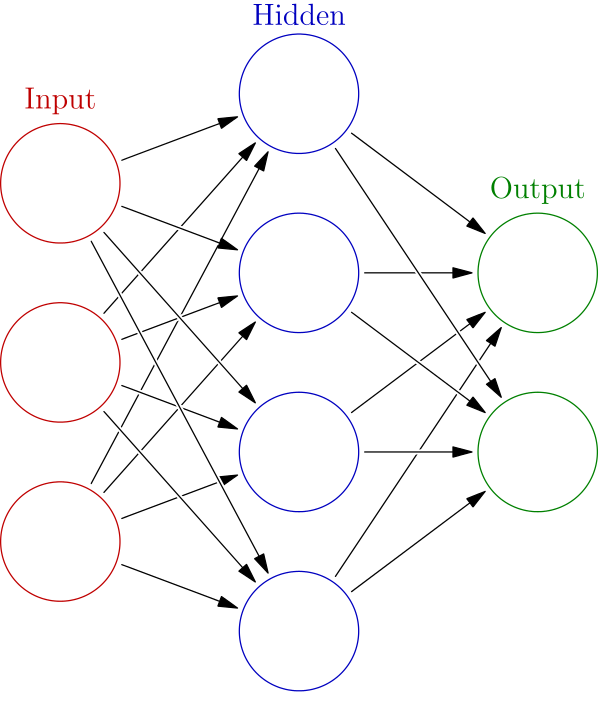
\includegraphics[width=.3\textwidth]{nn}
	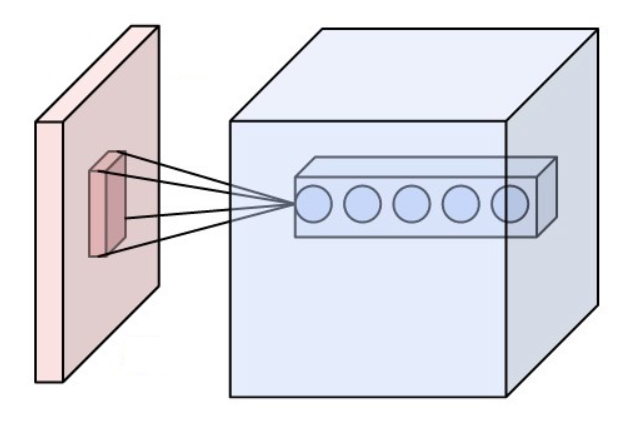
\includegraphics[width=.5\textwidth]{Conv_layer}
	\caption{Left: a very simple neural network with 3-dimensional input (red),  one hidden layer with 4 hidden units (blue),  and 2-dimensional output (green). Right: A pictorial representation of a convolutional layer of a neural network.}
\end{figure}
A \textbf{neural network} is a network of \textbf{neurons}, which represent units of computation organized in \textbf{layers}. (see Figure 2). For example, say we have input 3-dimensional input $\vec{x} = [1,2,3] $. Each of those values would be passed to the input neurons in Figure 1. Then, the first set of black arrows moves the input layer to the hidden layers by multiplying them by some weights and summin]g them together. This is equivalent to multiplying the $3 \times 1$ vector $\vec{x}$ by a $5 \times 3$ matrix of weights, $W$. Then a nonlinear function $f$ is applied elementwise to the 5 dimensional vector $W\vec{x}$. This nonlinear function increases the complexity of the space the neural network can explore, and is usually $f(x) = \tanh(x)$. This process is repeated with the output layer to achieve a $2\times 1$ output vector. In total, the computational process of the neural network can be captured by the equation
$$\vec{output} = f(W^2(f(W^1(\vec{input}))))$$
where $\vec{input}$ is the $3 \times 1$ input data, $W^1$ is the $5 \times 3$ weight matrix for the first layer, $W^2$ is the $2 \times 5$ weight matrix for the second layer, $f$ is an elementwise nonlinear function, and $\vec{output}$ is the $2\times 1$ output vector. The \textbf{activation of a layer}, $F^\ell$ is the intermediary result of running a given input through the network. For example, the activation of the first layer $F^1$ is 
$$F^1= f(W^1(\vec{input}))$$
A \textbf{convolutional neural network} is a neural network is at least one convolutional layer. This neural architecture is inspired by the organization of the human visual cortex, which small regions of neurons are aggregated into a single value. A convolutional layer is a layer that takes a small window of the input data and computes a single value for that region. For example, a \textbf{max pooling} convolutional layer simply computes the maximum value found for a given window (see Figure 2).

Through many layers and complex nonlinearities, a neural network with only a single hidden layer can approximate any function \cite{hornik1991approximation} with sufficient weights. But how are these weight matrices $W^i$ constructed?  This requires \textbf{training} the neural network to configure these weight matrices. In general, this is achieved by feeding it labeled data, $(x,y)$ (with $x_i \in \mathbb{R}^3$ and $y_i \in \mathbb{R}^2$ for our example) and initializing the weights as random. Then, for each observation $x_i$, a prediction $\hat{y}$ is computed by running $x_i$ through the network:
$$\hat{y} = f(W^2(f(W^1(x_i))))$$
Then the error in the network can be computed as the difference between the prediction and the actual output:
$$E(x_i) = (\hat{y} - \hat{y})^2$$
The weights can then be updated by descending the gradient of the error using \textbf{backpropagation}.  A review of the backpropagation algorithm is beyond the scope of this paper, but for a full overview, see \cite{rumelhart1988learning}.

For the purposes of image processing, the input data is raw images $x \in \mathbb{R}^{1000 \times 1000 \times 3}$ assuming they are 1000 pixels by 1000 pixels and are colored. The output $y$ used to trained the network is often labels corresponding to what the image is of, such as: $$y \in \{\text{elephant}, \text{doughut}, \cdots, \text{child},\text{apple}  \}$$
A well documented phenomenon of applying DCNNs to image processing is that lower level layers correspond to pixel or edge level information, and as you look at higher level layers, you get more high order structure. As information passes from the input image pixels to the output classifier, the ``scale'' of that projection increases. For example, layers towards the input correspond to local pixelated regions, edges and neighboring contours. Layers towards the output correspond to global structure, groups of aggregated edges, etc.  The work presented in this paper takes advantage of this important fact.  We will refer to this phenomenon as the visual hierarchy phenomenon (VHP).
\section{Matrix factorization}

Another famous approach for finding the low-rank approximation of a matrix $X$ is  matrix factorization, which aims to find an $A$ and $S$ such that $X \approx AS$ as shown in Figure \ref{nnmf}. Typically, for a input matrix $X \in \mathbb{R}^{n \times m}$ the size of the inner dimension, $k$, is specified ahead of time (such that $A\in \mathbb{R}^{n \times k}$ and $S\in \mathbb{R}^{k \times m})$. Since $k$ is chosen such that $k < \min(m,n)$ we have the was $\operatorname{rank}(AS) = k$, which gives us our low-rank approximation of $S$.

As discussed further in Section \ref{image}, the constraints imposed upon $A$ and $S$ result in different interpretations of the result. For example, constraining the columns of $S$ to be a unary vectors, where one element is equal to one and the other elements are zero, results in the Vector Quantization. Or constraining the columns of $A$ to be orthonormal and the rows of $S$ to be orthogonal to each results in Principal Component Analysis. 

In this thesis, I will focus on a third class of constraints, whereby $A$ and $S$ must be non-negative matrices. This constraint is shown to yield a parts-based approach, which is consistent with a ``topic model'' notion \cite{lee1999learning}." What results is a family of algorithms dubbed \textit{non-negative factorization} or NNMF.

 NNMF was first employed by Paatero and Tapper \cite{paatero1994positive} but was made popular by Lee and Seung \cite{lee1999learning}.
\begin{figure}[h]
	\label{nnmf}
	\centering
	\begin{blockmatrixtabular}
		\valignbox{\fblockmatrix[1.0,0.8,0.8]{1.2in}{0.8in}{$X$}}&
		\valignbox{\mblockmatrix                    {0.15in}{0.8in}{$\approx$}}&
		\valignbox{\fblockmatrix       [0.8,1.0,0.8]{0.6in}{0.8in}{$A$}}&
		\valignbox{\mblockmatrix                    {0.15in}{0.6in}{$\times$}}&
		\valignbox{\fblockmatrix       [0.8,0.8,1.0]{1.2in}{0.6in}{$S$}}&
	\end{blockmatrixtabular}
	\caption{A visual representation of the non-negative matrix factorization}
\end{figure}

The problem of finding such a factorization can be formulated as finding a non-negative $A$ and $S$ that minimize the error 
\begin{align}F = ||X-AS||^2
\end{align}
While this optimization problem is not convex in both $A$ and $S$, it is convex in one of them. So for a given, fixed $S$, we can find the optimal $A$ by setting the gradient equal to zero. Since $||X-AS||^2 = \langle X-AS, X-AS \rangle= X^TX - 2X^TAS + (AS)^T(AS)$ we have
\begin{align*}
\frac{\partial F }{\partial A} ( X^TX - 2X^TAS + (AS)^T(AS)) = 0\\
\text{implies }S^TAS = 2X^TS
\end{align*}
which is to say $\frac{X^TS}{S^TAS}=1$ at the optimal $A$. This equality gives us the below multiplicative update algorithm. 

\begin{algorithm}[H]
	\KwIn{k=0; Initialize $A^0, S^0$}
	\Repeat{Stopping condition}{
		\begin{align*}
		A^{k+1} &= A^k \circ \frac{XS^k}{A^k(S^k)^TA^k}\\
		S^{k+1} &= S^k \circ \frac{XA^{k+1}}{S^k(A^{k+1})^TA^{k+1}}\\
		k &= k+1
		\end{align*} 
	}
	\caption{Multiplicative Update}
\end{algorithm}

This optimization scheme naturally leads to a convex optimization function, so the above algorithm can simply be iteratively applied (until for given $T$ we have $k>T$ or for a given $\epsilon>0$ we have $||X-AS||^2 \leq \epsilon$).
\begin{theorem}
	The Euclidean distance $||X-AS||^2$ is non-increasing under the updating rules of Algorithm 1.
\end{theorem}

A key benefit of non-negative matrix factorization is that its results are very interpretatable. For a given factorization $X \approx AS$, we can think of the $k$ rows of $S$ as a basis $(b_1,b2_,\cdots,b_k)$ for the rows of $X$. Under this interpretation, the row of $A$ give us the linear combination used to form the corresponding row in $X:$
$$X_{i,} = \sum_{j= 1}^k A_{i,j} \times S_{j,}$$
This interpretation is directly applicable to the notion of ``geons as topics'' put forward in Section \ref{interp}. In this thesis, we will focus on NNMF as the central algorithm and we will explore how NNMF can be used to build a theory of visual perception.

\section{Comparison of NNMF and SVD}
Both SVD and NNMF as discussed above can yield a matrix factorization, which can be interpreted as a ``topic model'' (see Chapter \ref{natlang} for a more in depth explanation of this). Since NNMF already learns a matrix factorization, it is clear how this can be interpreted as a topic modelling scheme. 

Recall that SVD factorizes a matrix into the product of a unitary matrix, a singular values matrix and another unitary matrix
$$X \approx U \Sigma_k V^T$$
In Section \ref{section:svd}, for a given $X \in \mathbb{R}^{n \times m}$ we referenced the so called \textit{full} SVD. Under this framework, we have $U \in \mathbb{R}^{n \times n}, \Sigma  \in \mathbb{R}^{n \times m}$ and $V \in \mathbb{R}^{m \times m}$. Under the full SVD, it is somewhat unclear how to interpret the factorization as a topic modelling scheme as we did for NNMF. 

So we turn to another way to representing SVD, the \textit{compact} SVD. If you recall from Section \ref{section:svd}, under the full SVD the singular value matrix $\Sigma$ is 
$$\Sigma_k = \begin{bmatrix}
\sigma_1  & 0     & \cdots      &0       &   \cdots & 0   \\
0  & \sigma_2 & \cdots & 0    &  \cdots & 0    \\
\vdots  & \vdots & \ddots & \vdots &  & 0   \\
0 & 0 & \cdots & \sigma_k  & \cdots & 0  \\
\vdots  &     \vdots    && \vdots & \ddots & \vdots  \\
0 & 0      &      \cdots  &0      & \cdots & 0 
\end{bmatrix} \in \mathbb{R}^{n \times m}$$
where $\sigma_i$ are the singular values. An identical way to represent the same information is by having $\Sigma_k \in\mathbb{R}^{k \times k }$.  The all zero last $n-m$ rows of the previous representation of $\Sigma_k$ made the last $n-m$ columns of $U$ and the last $n-m$ rows of $V^T$ all zero, we can simply remove those columns and rows respectively and equivalently get  
$$X \approx U \Sigma_k V^T$$
with  $U \in \mathbb{R}^{n \times k}, \Sigma  \in \mathbb{R}^{k \times k}$ and $V \in \mathbb{R}^{m \times k}$. From this representation, an analogy to NNMF's topic model $X \approx AB$ can be formed by having $A = U\Sigma, B = V^T$ or $A = U, B=\Sigma V^T$ (here I use $A = U\Sigma, B = V^T$ WLOG). Now I conduct a horserace between compact SVD and NNMF. The hypothesis is that although SVD is much closer to a global minimum in the optimization scheme, the non-negativity constraints endow NNMF with a better ability to form topic models.
\subsection*{Results}
To compare the semantic coherence of the topics learned by SVD and NNMF, I compute the NNMF factorization and compact SVD factorization as described above. Then for each topic $(k=10)$, I show the top 20 highest magnitude words. I repeat this process for two datasets, which are further discussed in the Appendix. These words are shown in Figure \ref{fig:svdnnmf}.
\begin{figure}[h]
	\label{fig:svdnnmf}
	\centering
	\hspace*{-1.5in}
	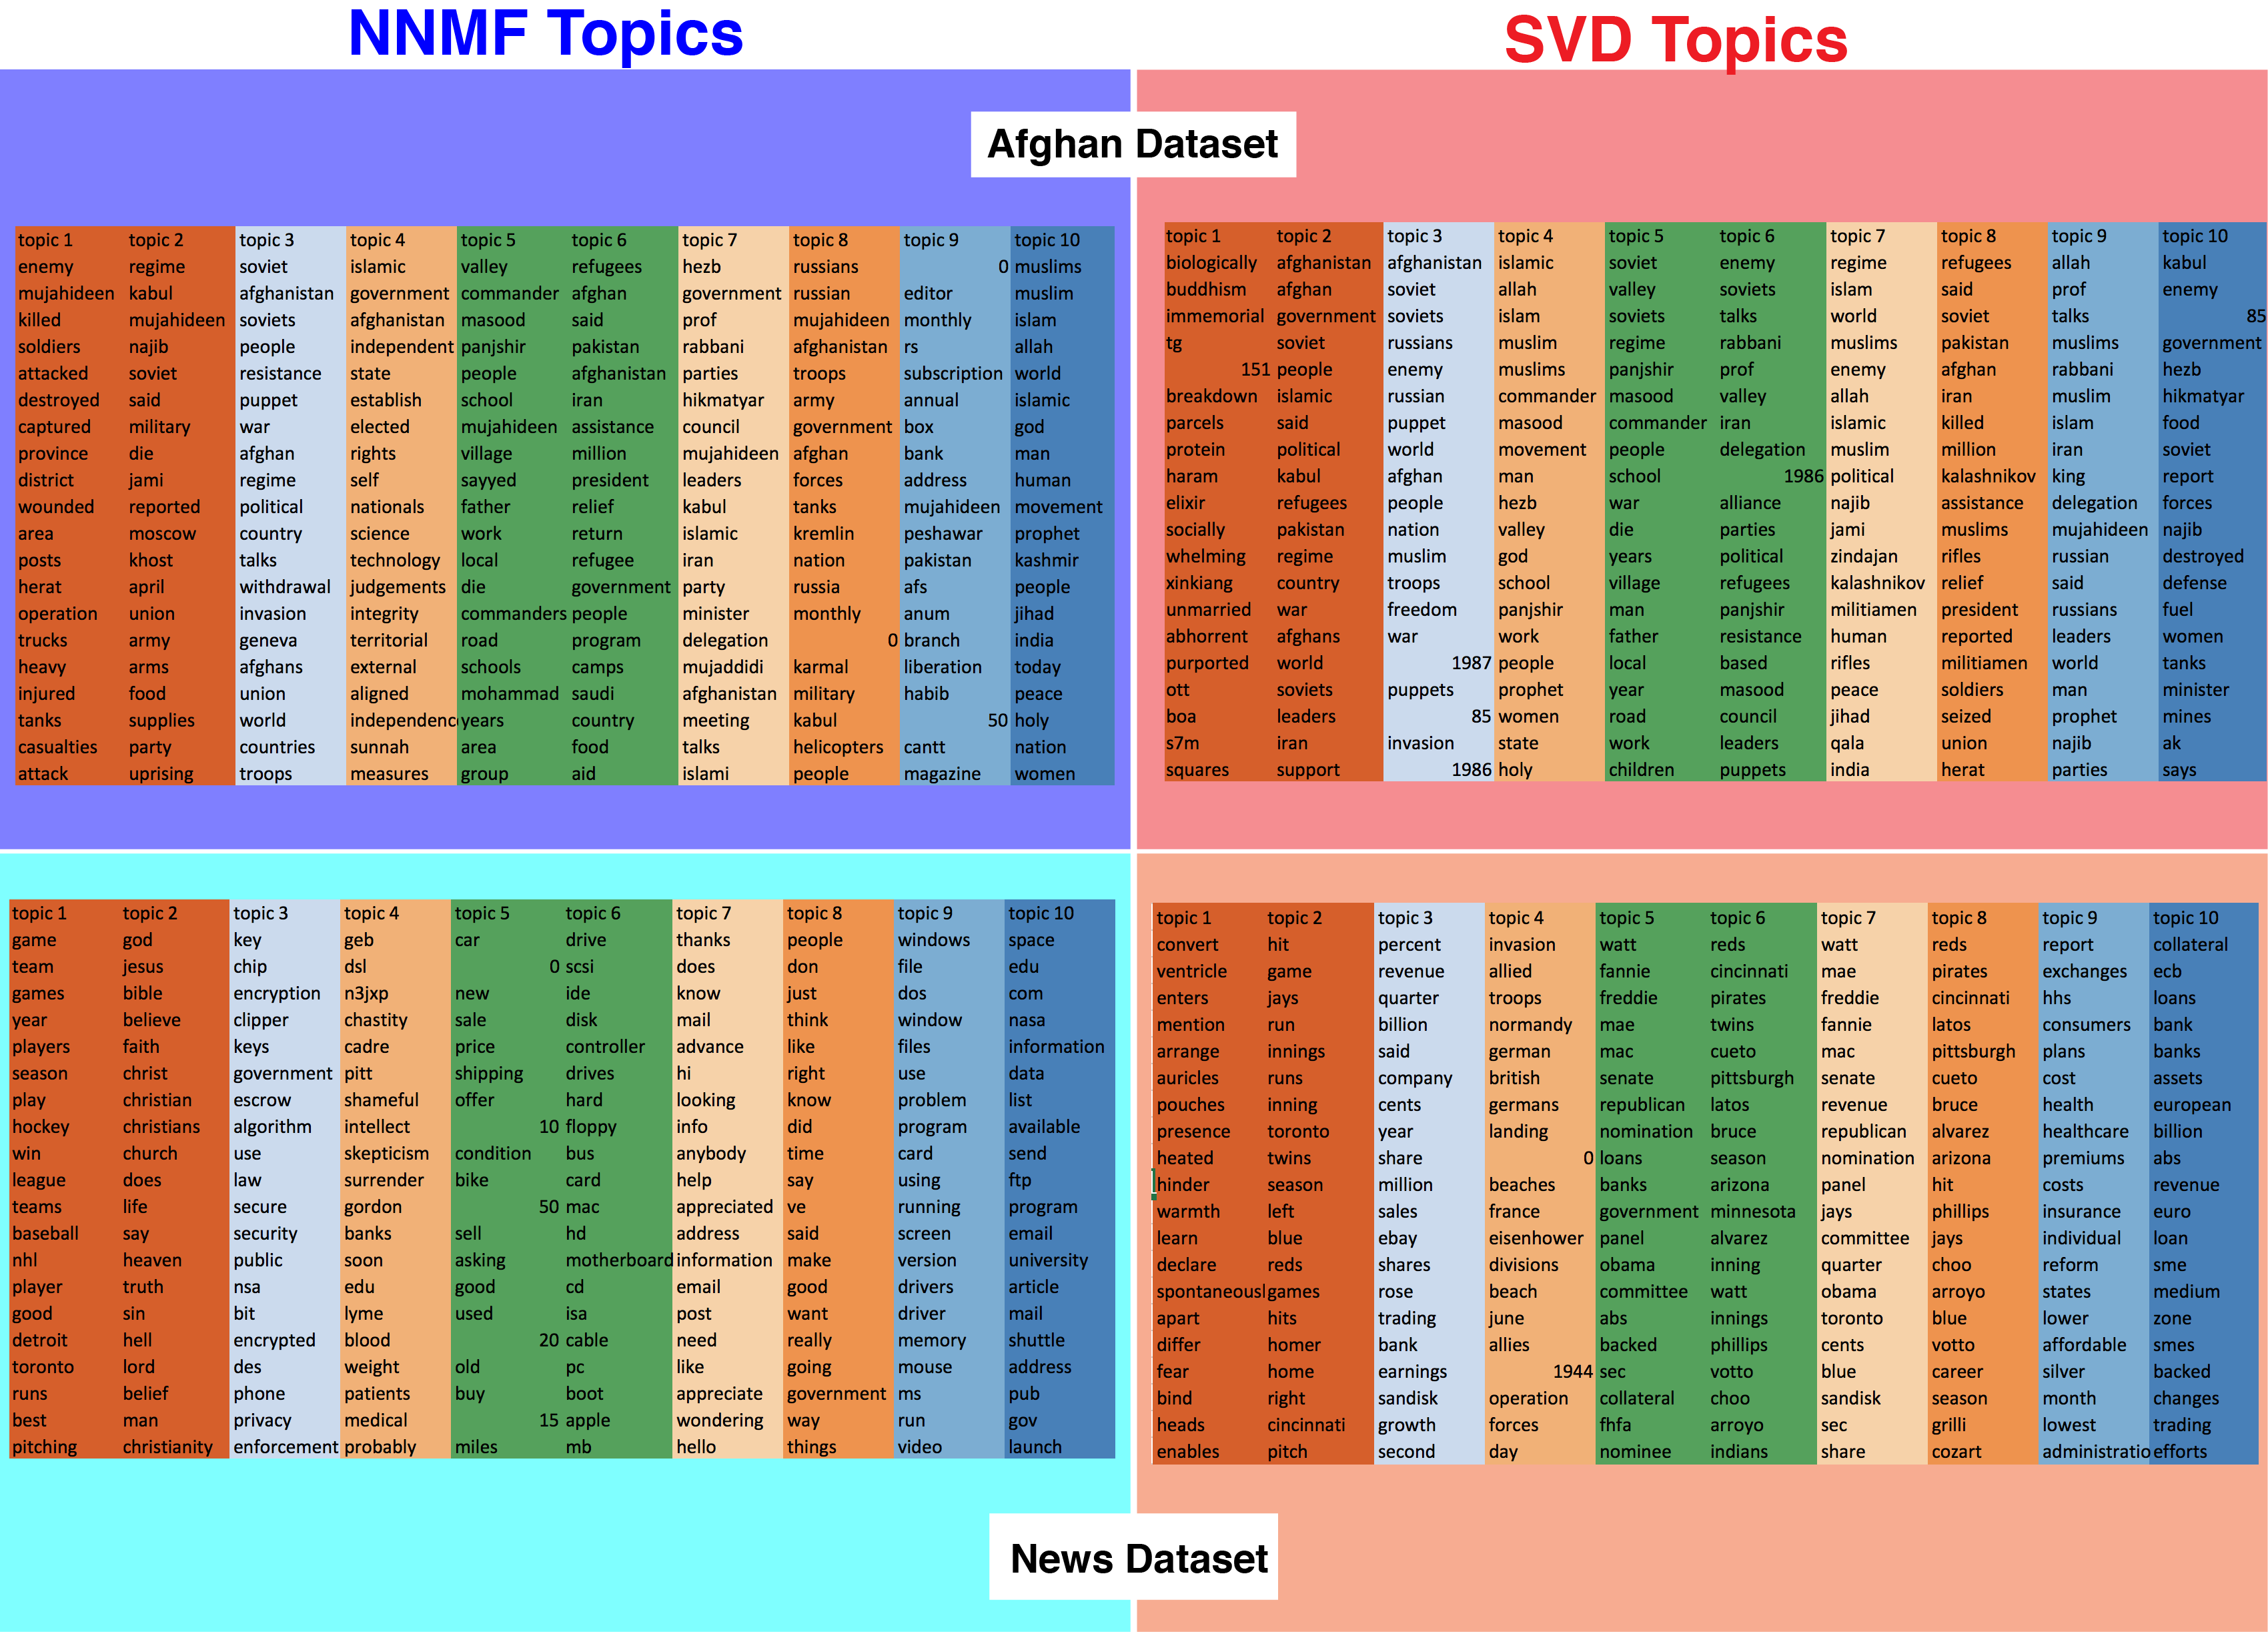
\includegraphics[width=1.4\textwidth]{imps/imps}
	
	\caption{The top words for NNMF  (left column in blue) and compact SVD (right column in red) factorizations of two data sets, Afghan (top) and News (bottom).}
\end{figure}
By inspection, one can see that the topics learned by NNMF correspond to semantically cohesive topics, while the topics learned by SVD do not. This is partially due to the fact that the SVD contains negative entries, and there is no direct intepretation to negative entries in a topic vector. This provides experimental evidence that NNMF is the correct factorization for tasks that care about semantically coherent topics.
\end{chapter}
\begin{chapter}{Types of Data}
	We have defined several algorithmic approaches for the automated understanding of any real valued matrices. In this chapter, we explore how important types of media and data can be represented as real valued matrices. Each section will focus on NNMF as the lens for analysis, and will describe how NNMF can be interpreted in each domain. 
\section{Image}
\label{image}

Because visual object recognition is the foundation of many of the cognitive theories discussed here, it makes sense to think about representing images as data. Because of how computers and digital cameras represent images, they are perhaps the most well suited for representation as data. For gray scale, an image is just a $w \times h$ matrix, where $w$ is the width of the image and $h$ is the height of the matrix. For color, an image is a triple $\{R,B,G\}$ where $R,B,G \in \mathbb{R}^{w \times h}$ correspond to red, blue and green intensities in the image, respectively.
\begin{figure}[h]
	\label{fig:face}
	\centering
	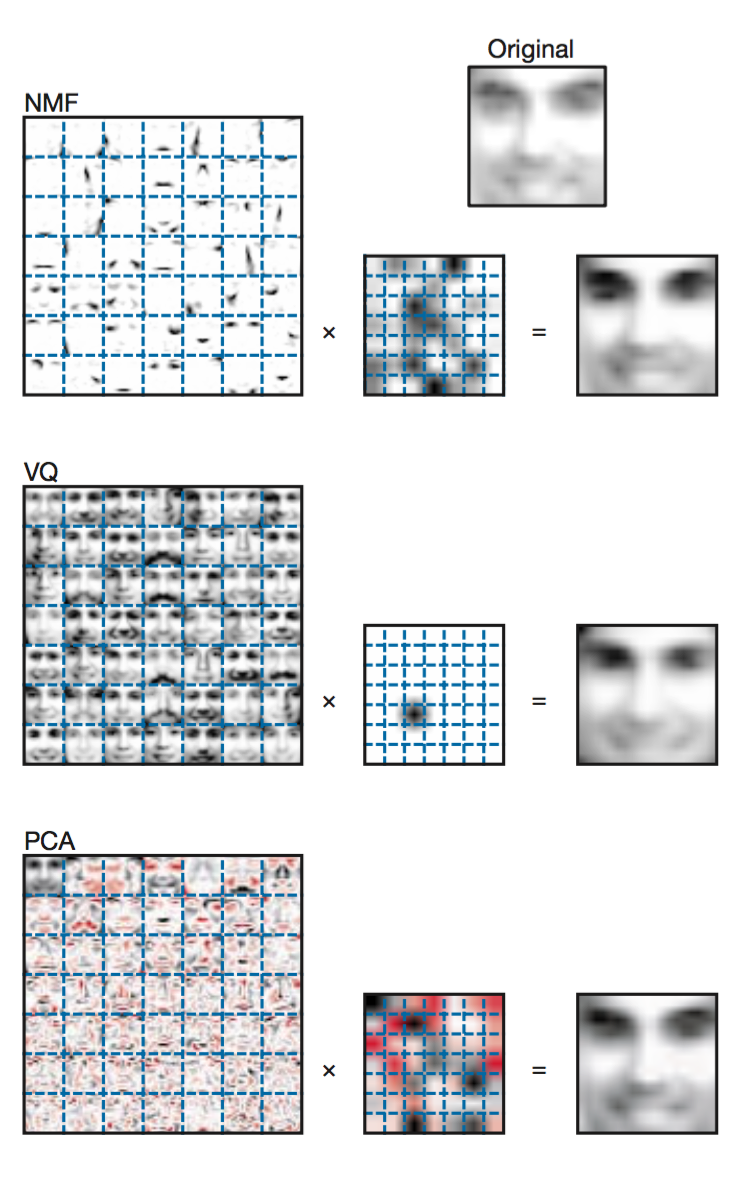
\includegraphics[width=6.2cm]{image}
	\caption{A comparison of the basis vectors learned for NMF, VQ and PCA. Adapted from \cite{lee1999learning}}
\end{figure}
The canonical demonstration of NNMF's ability to learn a parts-based representation utilizes a dataset of faces, $X$, with a row corresponding to a given image and the columns corresponding to a flattened vector representation of the matrix. Lee and Seung compare the NNMF factorization of this corpus with vector quantification (VQ) and principal component analysis (PCA). Indeed all three methods attempt to factorize $X$ into two matrices $A$ and $S$: the only difference is the constraints imposed on $A$ and $S$. As we have seen, NNMF does not allow nonnegative entries in either $A$ and $S$. For VQ, each column of $S$ is constrained to be a unary vector. And finally PCA contrains the colums of $A$ to be orthonormal and rows of $S$ to be orthogonal to each other \cite{lee1999learning}.

As can be seen in Figure \ref{fig:face}, the bases each approach learns is radically different. VQ learns a basis of prototypes, where each basis itself is an entire face, and each row of $X$ is a linear combination (i.e. addition and subtraction) of these protofaces. Alternatively, PCA learns a basis of `eigenfaces,' which correspond to ``distored'' versions of complete faces \cite{turk1991eigenfaces}. Instead of learning a``holistic'' representation of the faces like VQ and PCA, NMF learns a parts-based model, where the rows of $S$ correspond to discrete components of a face. 

\section{Sound}
Despite not being as discrete as images or graphs, sound also can be represented in a high structured way. There have been many approaches to do so. Perhaps the most success is the Deep Speech models, which feed speech snippets into a RNN paired with a language model for real time dictation \cite{amodei2015deep,hannun2014deep}. These Deep Speech systems represent sound as follows. An utterance $x$ is a time series of length $T$	sliced into time intervals $t$. For each time interval, the utterence is represented as a vector of audio features, $\vec{x_t}$. Hannun et al, in their famous Deep Speech neural model, use spectrograms as features, such that $\vec{x_{t,p}}$ is the power of the $p$th frequency bin the the audio frame at time $t$ \cite{hannun2014deep}.

Another approach is to take the modulus of a given signal's the STFT as treat that spectrogram  $X$ as a matrix to be factorized \cite{kawamoto2000estimation,krause2015non}. NNMF is particularly useful in this domain because the source components (the results of the factorization) are also interpreted as spectrograms, which must have non-negative entries. 

Holzapfel et al. do what is perhaps most organic given a corpus of sound documents. With inner dimension $k=10$, they find that the topics correspond to traditional genres of music \cite{holzapfel2008musical}. In addition, since the factorization yields sonic embeddings for each genre, the authors achieve a data driven notion of similarity between genres  (see Figure \ref{fig:sound}). 
\begin{figure}[h]
	\label{fig:sound}
	\centering
	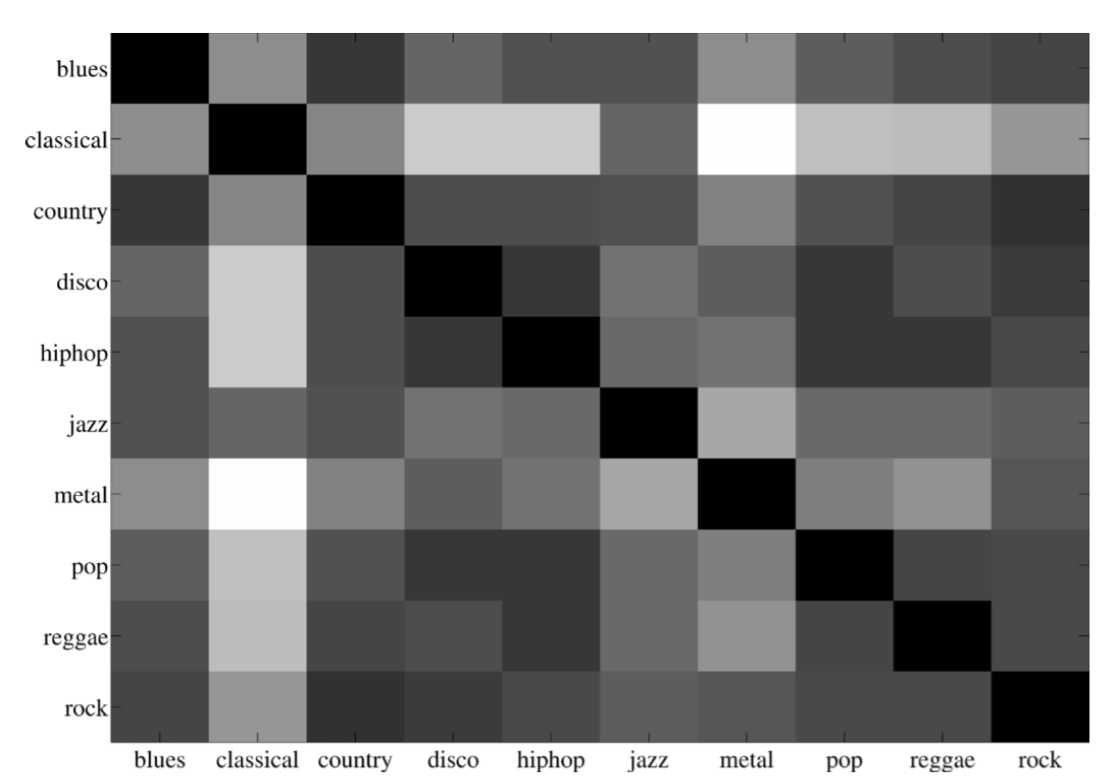
\includegraphics[width=12.2cm]{genre}
	\caption{Pairwise comparison of music genres. Adapted from \cite{holzapfel2008musical}}
\end{figure}
\section{Graph}
Since a network of edges and vertices $G=(V,E)$ can be represented as an \textit{adjacency matrix} $A \in \{0,1\}^{|V| \times |V|}$ with $A_{i,j} = 1$ if $(i,j) \in E$ and $A_{i,j}=0$ otherwise, graphs are another domain well suited for low dimensional representations. \footnote{For now, we will work with unweighted, undirected graphs, although these results generalize to other types of graphs as well.} Factorizing this adjacency matrix is equivalent to clustering the graph, which is a central problem to graph theory \cite{ho2008nonnegative}.
A given clustering $C = \{C_1, C_2, \cdots, C_k\}$ of a graph is a partition of the vertices and can be evaluated based on its \textit{connectivity}:
$$\text{connectivity}(G,C) = \frac{\#\{(i,j)\in E | (i,j) \in C\} + \#\{(i,j)\not\in E | (i,j) \not\in C\}}{|V|^2}$$
The clustering $C$ can be formulated as a membership matrix $M \in \{0,1\}^{n \times k}$ with $M_{ir}=1$ if $i \in C_r$ and $M_{ir}$ if $i \not\in C_r$. Thus, the connectivity of $G$ under $C$ as defined above can be rewritten:
\begin{align*}\text{connectivity}(G,C)  &= 1-\frac{\sum_{i,j} \left(A_{ij} - \sum_{r=1}^k M_{ir}M_{jr}\right)^2}{|V|^2}\\
&=1-\frac{||A-MM^T||^2_F}{|V|^2}
\end{align*}
Thus finding a clustering $C$ that maximizes the connectivity is equivalent to the minimization problem 
$$\min_{M \in \{0,1\}^{n\times k}} ||A-MM^T||^2_F$$
However, finding one such $M$ is NP-Complete \cite{vavasis2009complexity}. So we can relax the constraints to try to solve an easier problem we are more used to 
$$\min_{M \in \mathbb{R}_{+}^{n\times k}} ||A-MM^T||^2_F$$
which just the standard optimization for non-negative matrix factorization for the symmetric case. Since the $M$ we are solving for in this case is no longer binary, but rather contains reals, it is considered a \textit{weak membership matrix}. That is, the larger $M_{i,j}$, the stronger membership of vertex $i$ in cluster $j$. 
\section{Natural Language}
\label{natlang}
With the vast amount of digital text being generated across the internet, methods for understanding and processing corpora of human language become necessary. Across mathematics and computer science, many techniques have been put forward that allow one to understand a body of text far too large to read herself. A successful method in this domain is \emph{topic modelling}, whereby semantically cohesive subgroups of words can be identified. In particular, let $\mathcal{C} = \{d_1,d_2,\cdots, d_n\}$ be a collection of documents with a vocabulary $\mathcal{V}$. A \emph{topic}  $t_i$ is a vector over the words in the vocabulary that represents a coherent high level notion in the corpus:
$$t_i = \{v^i_1, v^i_2, \cdots, v_m^i\}$$
where $m$ is the size of the vocabulary. Topic modelling offers a powerful tool for understanding large amounts of text because they can discover latent semantic structure within text. 

There are two primary techniques for learning these topics $t_i$. The first is LDA, a generative Bayesian statistical model which views each document $d_j$ as a mixture of various topics.
The second is non-negative matrix factorization, which aims to factor the document/word matrix into a document/topic and a topic/word matrix \cite{lee1999learning, blei2012probabilistic}. The focus of this thesis will be NNMF, because of its relation to linear algebra, and its deep visual and conceptual intuition. 

Given our $n$ documents with vocabulary $\mathcal{V}$ of size $m$, we construct a matrix $X \in \mathbb{R}^{n\times m}$ where $X_{i,j}$ is the number of occurences of word $j$ in document $i$. For a given inner dimension $k$, we seek to factor $X$ into two matrices $A$ and $S$ such that
$$X \approx AS$$
where $A \in \mathbb{R}^{n\times k}$ is the document/topic matrix and  $S \in \mathbb{R}^{k\times m}$ is the topic/word matrix. When we impose that $A$ and $S$ must be non-negative, a strong intuition emerges. In particular, the $(i,j)$th entry of $A$ corresponds to the proportion of topic $j$ in document $i$ and the $(i,j)$th entry of $S$ corresponds to the relevance of word $j$ in topic $i$.

To gain some visual intuition into the interpretations of $A$ and $S$, consider Figure \ref{fig:tmex}. The rows of $S$ give us the word break down of each topic, which is shown on the left column under Topics. Then each document can be represented as a weighted combination of topics.
\begin{figure}[h]
	\label{fig:tmex}
	\centering
	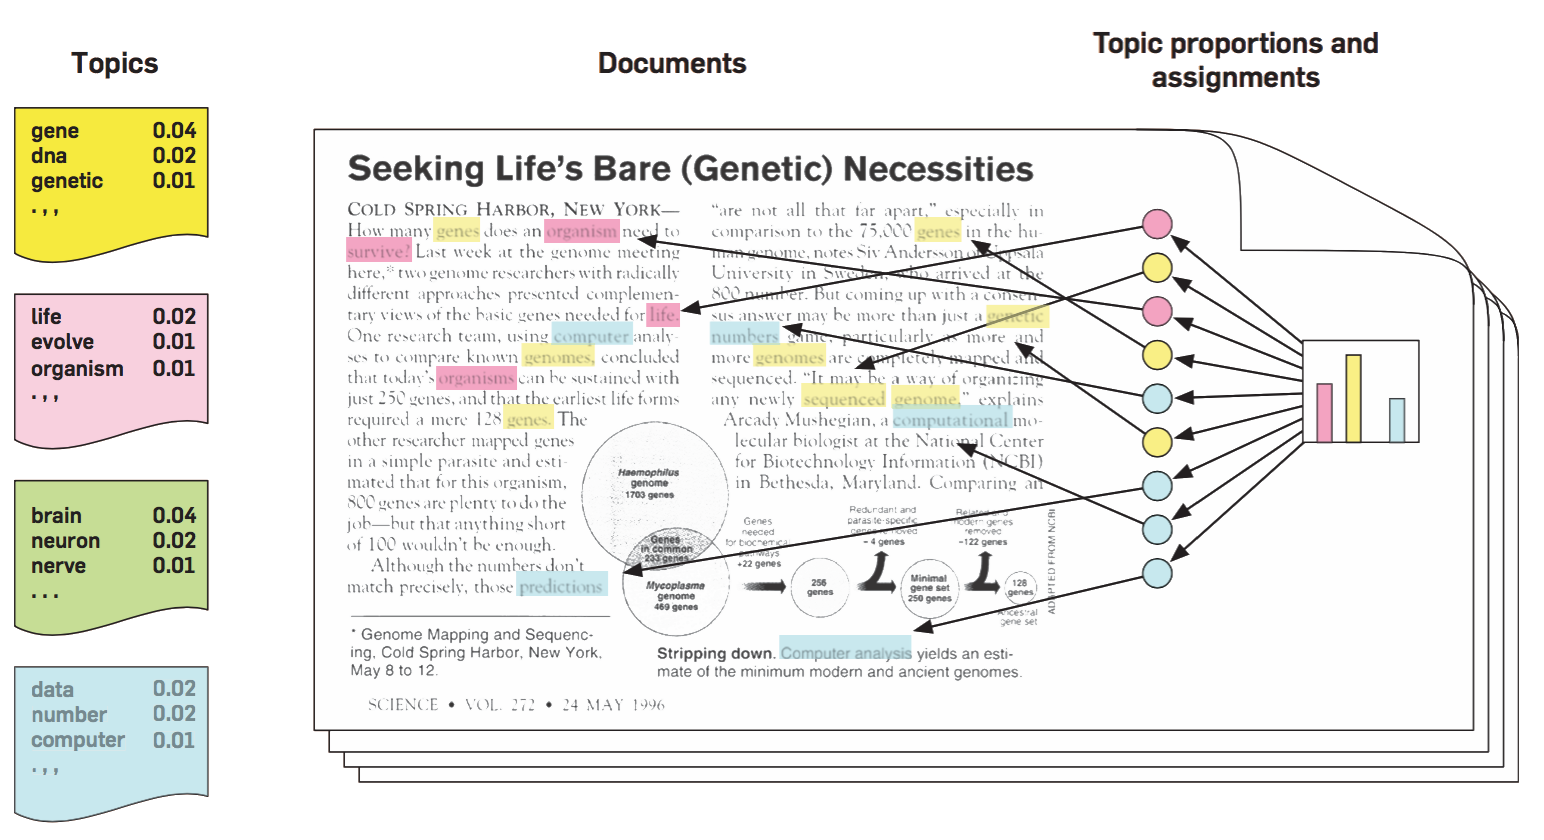
\includegraphics[width=16.2cm]{tmex}
	\caption{A visual interpretation of topic model on text. Adapted from \cite{blei2012probabilistic}}
\end{figure}

\end{chapter}



\begin{chapter}{Manifold Learning as NNMF}
	\label{supervised}
	
	\section{Motivation}
	The standard NNMF has several simplistic assumptions that reduce its robustness as a general model for human understanding. 

	\subsection*{Manifold Smoothness}
	First, standard NNMF only considers the data's euclidean embedding, but does not consider the inherent geometry of the data space \cite{cai2008non}. However, there is a growing body of evidence that suggests that object recognition corresponds to a locally continuous manifold \cite{dicarlo2012does}. We represent this formally with the \textit{manifold assumption}, which states that ``if two observations $x_i$ and $x_j$ are close in the instrinsic geometry of the data distribution, then the representations of the two points in the new basis are also close to each other \cite{belkin2001laplacian, cai2008non}.''
	
	In other words, let  $f_\ell(x_i) = s_{i\ell}$ be the mapping function from original observation $x_i$ s onto the axis $a_\ell$, then we have if $|x_i - x_j| < \epsilon$ then $|f_\ell(x_i) - f_\ell(x_j) | < \delta$ for some $\delta$. We will measure the smoothness of the $f_\ell$'s along the geodesics in the underlying geometry of the data space and denote it $||f_\ell||^2_M$ \cite{cai2008non}. 
	
	Let $\mathcal{M} \subset \mathbb{R}^m$ be the underlying smooth manifold that generated our data. Then the ``natural choice'' for $||f_\ell||^2_M$ is 
	$$||f_\ell||^2_M = \int_{x \in \mathcal{M}} ||\nabla_\mathcal{M} f_\ell||^2 dP_X(x)$$
	where $\nabla_\mathcal{M}$ is the gradient of $f_\ell$ along $\mathcal{M}$ and the integral is taken over the data distribution $P_X$.
	
	Unfortunately, the underlying data manifold $\mathcal{M}$ is unknown, so we cannot compute $||f_\ell||^2_M$ directly. Instead, we discretely approximate it through a nearest neighbor graph of the data using techniques from manifold learning theory \cite{belkin2003problems} and spectral graph theory \cite{chung1997spectral}. 
	
	First we construct an edge weight matrix $W$ such that
	 $$W_{ij} = \begin{cases} 
	1 & \textrm{ if $x_i \in N_p(x_j)$ or $x_j \in N_p(x_i)$} \\
	0 & \text{otherwise} \\
	\end{cases} $$
	where $N_p(x_j)$ is the set of the $p$ nearest points to $x_j$. Next let $L$ be the graph Laplacian defined as $L=D-W$, where $D$ is the diagonal matrix of column sums of $W$ (i.e. $D_{ii} = \sum_j W_{ij}$). \cite{chung1997spectral}. We leverage $L$ to form a discrete approximation for $||f_\ell||^2_M$, since the graph Laplacian $L$ is a discrete approximation of the Laplace-Beltrami operator $\Delta_\mathcal{M}$ on the underlying data manifold \cite{belkin2003problems}. Following Cai et al's derivation \cite{cai2008non}, we get the following closed form for $\mathcal{R}_\ell$, the discrete approximation for $||f_\ell||^2_M$:
	\begin{align*}
\mathcal{R}_\ell &= \frac{1}{2} \sum_{i,j=1}^N (f_\ell(x_i)-f_\ell(x_j))^2W_{ij}\\
&=\sum_{i=1}^N f_\ell(x_i)^2 D_{ii}  - \sum_{i,j=1}^N f_\ell(x_i)f_\ell(x_j)W_{ij} \\
&= \sum_{i=1}^N v_{i\ell}^2 D_{ii}  - \sum_{i,j=1}^N v_{i\ell}v_{j\ell}W_{ij} \\ 
&= s_\ell^TDs_k - s_\ell^TWs_\ell \\
&= s_\ell^TLs_\ell
	\end{align*}
So $\mathcal{R}_\ell$ can be used to measure the smoothness of $f_\ell$ about the underlying geometry of the data space. So the matrix factorization that minimizes all the $\mathcal{R}_\ell$, which Cai et al denoted \textit{graph reguarized NNMF} or gNNMF, will maximize the smoothness of the mapping. The minimization of the  $\mathcal{R}_\ell$ is added to the energy function as follows
\begin{align}
\label{O:gNNMF}
\mathcal{O}_{\text{gNNMF}} &= ||X-AS||^2_F + \lambda \sum_{\ell=1}^k \mathcal{R}_\ell \\&=  ||X-AS||^2_F + \lambda \operatorname{Tr}(S^TLS)
\end{align}
The authors also put forward a multiplicative update algorithm that is non-decreasing in $\mathcal{O}_{\text{gNNMF}} $: 

	\begin{algorithm}[H]
		\KwIn{Initialize $A^0, S^0$}
		\Repeat{Stopping condition}{
			\begin{align*}
			A_{ij} &\leftarrow 	A_{ij} \frac{(XS)_{ij}}{(AS^TS)_{ij}}\\
			S_{ij} &\leftarrow 	S_{ij} \frac{(XA_\lambda WS )_{ij}}{(SA^TA + \lambda DS)_{ij}}\\
			\end{align*} 
		}
		\caption{Multiplicative Update for Graph Regularized NNMF}
	\end{algorithm}
	It's important to note that $W$ can be any matricial representation of the structure of the data. Here, Cai et al use $p$-nearest neighbor edge weight matrix, but are explicit in stating that this choice is arbitrary. If for whatever reason the data is known to exhibit structure in the form of some matrix $W'$, then the results above generalize to that matrix as well.
	\subsection*{Supervision}
	Canonical NNMF is unsupervised, which means the algorithm is designed to reveal latent structure from unlabeled data. Many times however, data is accompanied with labels. In this case, the alternative algorithmic objective is to assign new unobserved data into appropriate labels.
	
	As I briefly discussed in Section \ref{manifold}, the supervised formulation is inherently related to the problem of visual object recognition \cite{biederman1987recognition}. Objects can be thought of as both their class labels and their retinal activations (see Figure \ref{manifold}).
\begin{figure}[h]
	\label{manifold}
	\centering
	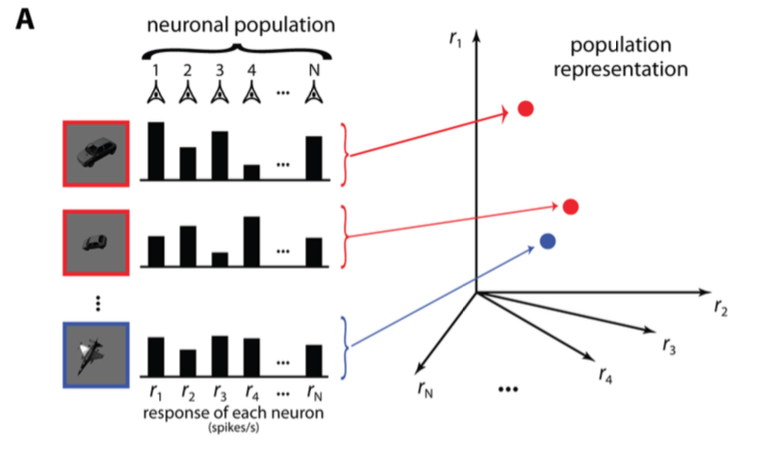
\includegraphics[width=.42\textwidth]{manifoldA}
		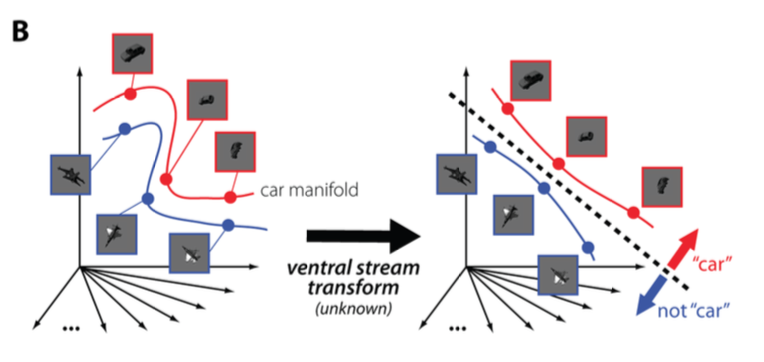
\includegraphics[width=.57\textwidth]{manifoldB}
	\caption{A: Supervised representation of object recognition; B: seperating hyperplane via ventral stream transform. Image adapted from \cite{dicarlo2012does}.}
\end{figure}	

	A core task in the object recognition problem is to understand how the brain creates a separating hyperplane in this high dimensional retinal representation of objects. A growing body of literature suggests that the primate ventral visual processing steam -- a region of cortical segments in the temporal and occipital lobes -- contains import circuits for object recognition \cite{gross1994inferior, dicarlo2012does, miyashita1993inferior, orban2008higher, rolls2000functions}. 
	
	Although the explicit algorithmic mechanisms of this ventral stream transform are still not yet known, in this section we will explore several analogies in the domain of NNMF. In particular, we will explore  the semi-supervised case, where only some of the data is labeled.  For semi-supervised NNMF (ssNNMF), the objective is similar to the unsupervised case. However, the known class labels can be incorporated into the model to improve classification performance \cite{lee2010semi}. We will explore an extension of NNMF where some of the class labels are known, and this information is used to enhance the performance of the NNMF. This ssNNMF  learns a one-versus all separating hyperplane for the observations \cite{lee2010semi} as follows.
	
   In addition to  $X \in \mathbb{R}^{n\times m}$ we also have a label matrix $Y \in \mathbb{R}^{n\times k}$, where $k$ is the number of classes and $Y_{i,j}$ is 1 if document $i$ is in class $j$ and 0 otherwise. 
	Given $B \in \mathbb{R}^{k \times r}$, a basis matrix for $Y$, and $L \in \mathbb{R}^{k \times n}$, a weight matrix to handle missing labels, then the energy function for SSNMF is as follows
\begin{align}
\label{O:ssMMMF}
\mathcal{O}_{\text{ssNNMF}} = ||(X-AS)||^2 + \lambda ||L \circ (Y-BS)||^2
\end{align}
	where $\lambda$ is a tradeoff parameter that governs the importance of the supervised term.
	
	In the same vein of Algorithm 1, this energy function yields a convex optimization problem solved by the following algorithm. 
	
	\begin{algorithm}[H]
		\KwIn{k=0; Initialize $A^0, S^0, B^0$}
		\Repeat{Stopping condition}{
			\begin{align*}
			A^{k+1} &= A^k \circ \frac{XS^k}{A^k(S^k)^TS^k}\\
			B^{k+1} &= B^k \circ \frac{(L \circ Y )S^k}{(L \circ B(S^k)^T)S^k}\\
			S^{k+1} &= S^k \circ \frac{(A^{k+1})^TX + \lambda B^T (L \circ Y)}{(A^{k+1})^TAS + \lambda B^T (L \circ BS)}\\
			k &= k+1
			\end{align*} 
		}
		\caption{Multiplicative Update for Semi-Supervised NNMF}
	\end{algorithm}
	I implemented this algorithm for the Afghan dataset, where the each of the documents corresponds to one of three groups, the results of which are shown in Figure \ref{fig:semi}. Here $k=3$, so each sunburst corresponds to the hierarchical model learned for each group. 
	\begin{figure}
		\label{fig:semi}
		\centering
		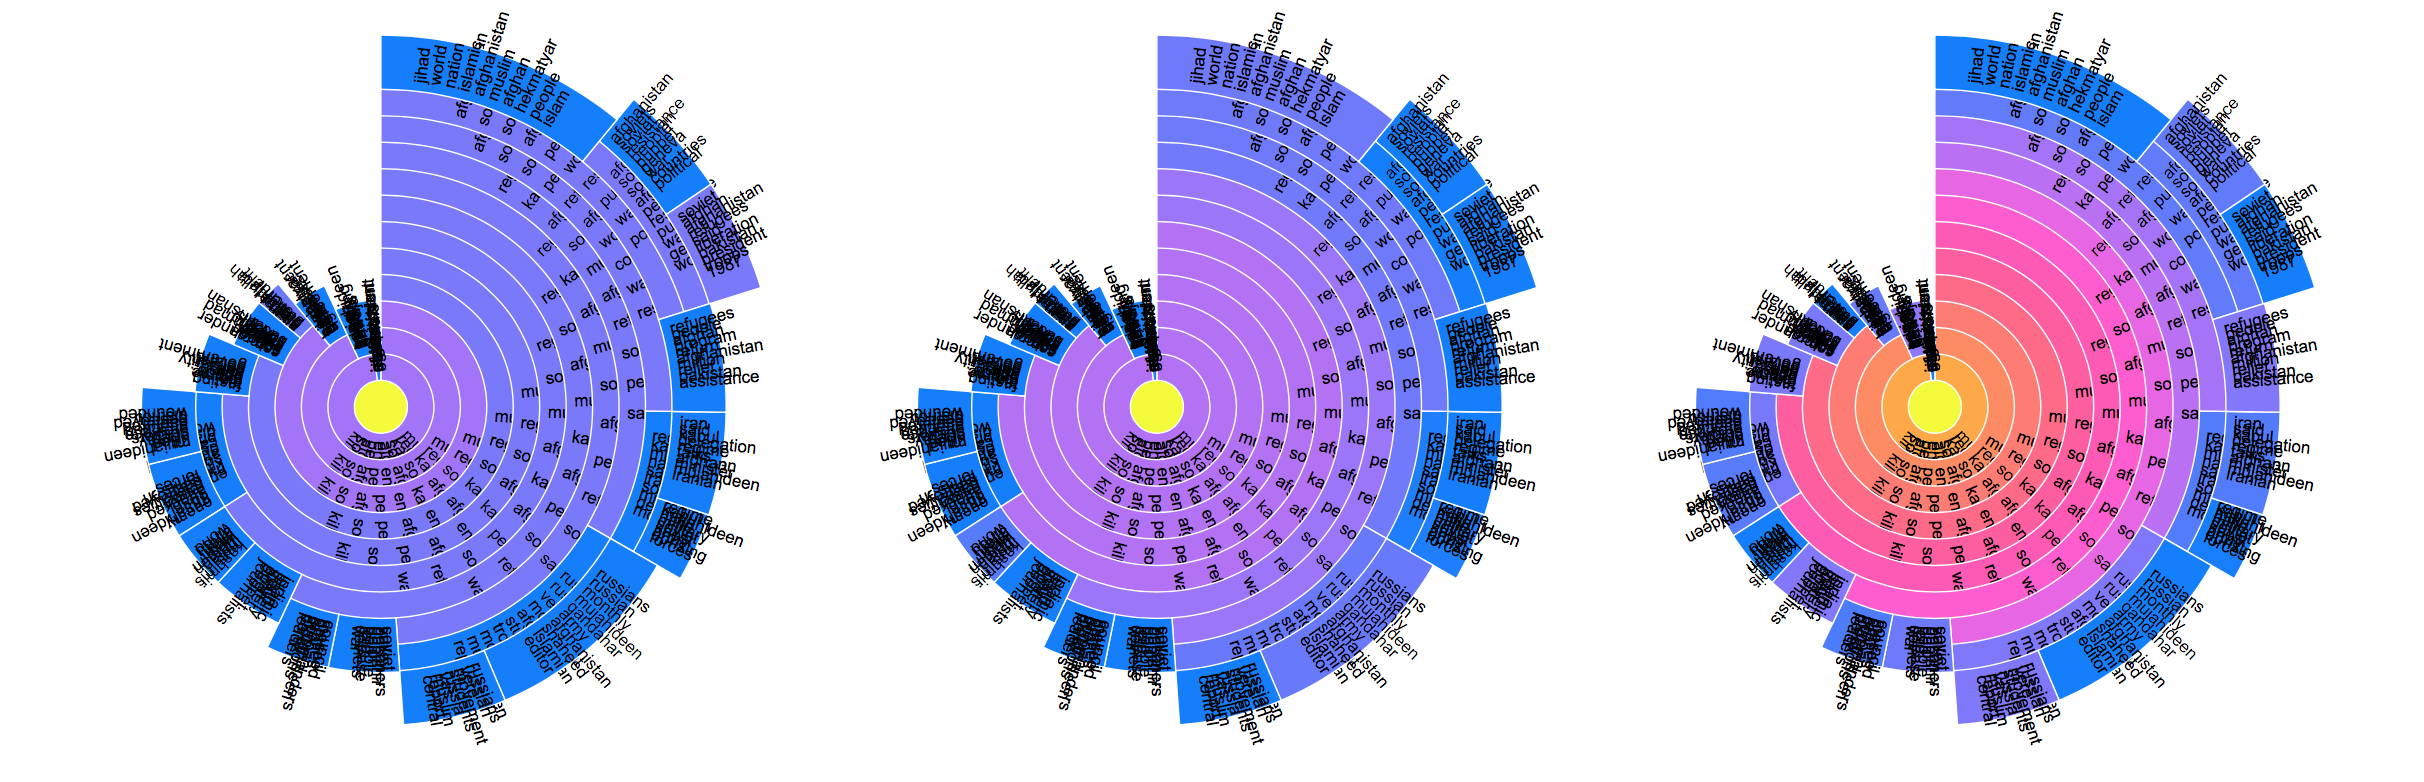
\includegraphics[width=7in]{semi-viz}
		\caption{ssNNMF by label}
	\end{figure}
	
	\section{Manifold NNMF}
	\label{mNNMF}
	I conclude this section by proposing a new NNMF that directly  combines the two methods discussed above, gNNMF and ssNNMF, to learn a supervised, locally smooth model. Inheriting from the energy functions \ref{O:gNNMF} and \ref{O:ssMMMF}, the energy function for Manifold NNMF is
	\begin{align}
	\mathcal{O}_{\text{manifold}} =  ||(X-AS)||^2 + \lambda_1 ||L \circ (Y-BS)||^2 +  + \lambda_2 \operatorname{Tr}(S^TLS)
	\end{align}
The formal analysis of this schema is beyond the scope of this thesis, but I hope its conclusion motivates future work in the development of a cognitively sound NNMF.
\end{chapter}
\begin{chapter}{Hierarchical Representation}
Many times, the data we wish to represent exhibits hierarchical structure. One such example is with the topics found in text data. Since topics correspond to semantic ideas, it makes sense that they would be organized into a hierarchy. For example, in the 20 News Group data set, there are two separate topics for the Cincinnati Reds and Toronto Blue Jays, two baseball teams. Thus one could think about a supertopic, baseball, that branches into the two topics the standard NNMF finds.
\section{Approach}
For a given document matrix $V$, we use the python library \texttt{scikitlearn} to decompose $V$ into document/topic matrix $W$ and topic/word matrix $H$ such that $$V \approx WH.$$ The  \texttt{scikitlearn} library contains a function \texttt{NMF} that performs the factorization: 


$$\texttt{nmf = sklearn.decomposition.NMF(n\_components=k).fit(X)}$$


The \texttt{scikitlearn} NNMF implementation uses alternating gradient descent with the following objective function to generate optimal guesses for $W$ and $H$.
$$c(H,W) = \tfrac{1}{2} ||X-WH||_{fro}^2 + \alpha \lambda ||W||_1 + \alpha \lambda ||H||_1 + \tfrac{1}{2} \alpha (1-\lambda) ||W||^2_{fro} + \tfrac{1}{2} \alpha (1-\lambda) ||H||^2_{fro}  $$
where $||\cdot||_{fro}$ is the Frobenius norm, $||\cdot||_{1}$ is the L1 norm, $\lambda$ is the L1 ratio and $\alpha$ is a free parameter \cite{nnmfimp}. For a more information, see the \texttt{scikit learn} documentation \cite{nnmfimp}.

From the $N$ topics $t_n$ for $n \in \{1\cdots N\}$\footnote{observe that $t_n$ is simply the $n$th row of $H$}, we populate an adjacency matrix $A$ where $$A_{i,j} = \frac{T_i \cdot T_j}{||T_i|| \ ||T_j||}$$ is the cosine similarity between topics $i$ and $j$. We then define a \emph{threshold vector} $\sigma$ by sorting all the elements of $A$. $$\sigma = \{\sigma_1, \sigma_2, \cdots \sigma_{N^2} \mid0 \leq \sigma_{i} \leq \sigma_j \leq 1 \forall i \leq j\text{ and }\sigma_k \in A\}$$
We then create an array of graphs $A^{(k)}$ thresholded using the values of $\sigma$, such that  \[
A^{(k)}_{i,j} =
\begin{cases}
1 & \text{if } A_{i,j} >\sigma_k\\
0 & \text{otherwise.}
\end{cases}
\]
Observe that $A^{(1)}$ is the fully connected graph and $A^{(N^2)}$ is the completely disconnnected graph.
By looking at the connected components  of a given graph,
$$c(A^{(j)})=\{c^j_1, c^j_2,\cdots,c^j_i,\cdots,c^j_N\}$$
where $c_i =k$ means that the $i$th vertex is in the $k$th order component, we can formulate a tree structure (see Figure 1).
\begin{figure}
	\centering
	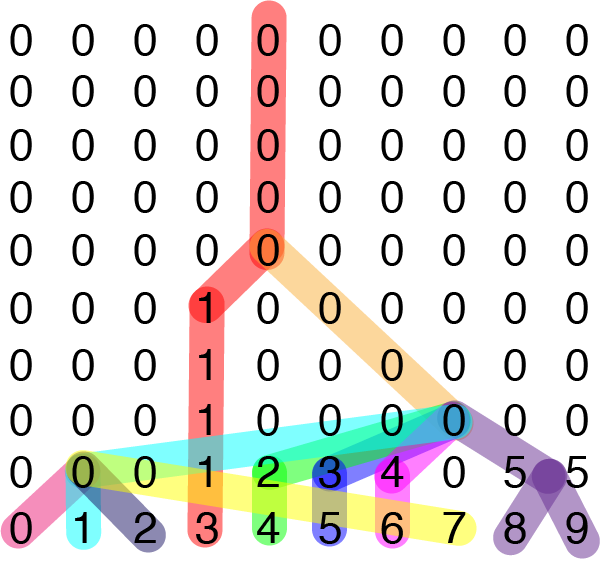
\includegraphics[width=.5\textwidth]{agglomeration}
	\caption{How the tree structure is formed for the connected component vectors}
\end{figure}
For example, say $N=8$ and we have
\begin{align*}
c(A^{(j)})=\{0, 0, 0 ,0, 1 ,1 ,1, 1\}\\
c(A^{(j+1)})=\{0, 0, 0 ,0, 1 ,1 ,2, 2\}
\end{align*}
This means that $A^{(j)}$ has two connected components, ordered 0 (with vertices 1,2,3,4) and 1 (with vertices 5,6,7,8) and that $A^{(j+1)}$ has three connected components, ordered 0 (with vertices 1,2,3,4), 1 (with vertices 5 and 6) and 2 (with vertices 7 and 8).  Thus there is a branch from the connect component 1 in $A^{(j)}$ to the connected componenets 1 and 2 in $A^{(j+1)}$. By greedily repeating this iterative algorithm starting with $A^{(1)}$ \footnote{which has by definition only a single connected component and so $c(A^{(1)})=\{0, \cdots, 0\}$} as the root, we produce the tree of topics. Observe that at this stage, all the leaf nodes correspond to actual topics $t_n$. We formulate the topic vectors for the parent nodes by additive percolating up the tree. That is, for a given parent topic $\tau$ with children $\tau_1, \cdots, \tau_k$ we simply have 
$$\tau =\sum_i \tau_i $$
The code that proceduralizes the above algorithm can be found in the \textbf{Building a hierarchy} section of the Appendix.
\section{Visualization}
\begin{figure}
	\centering
	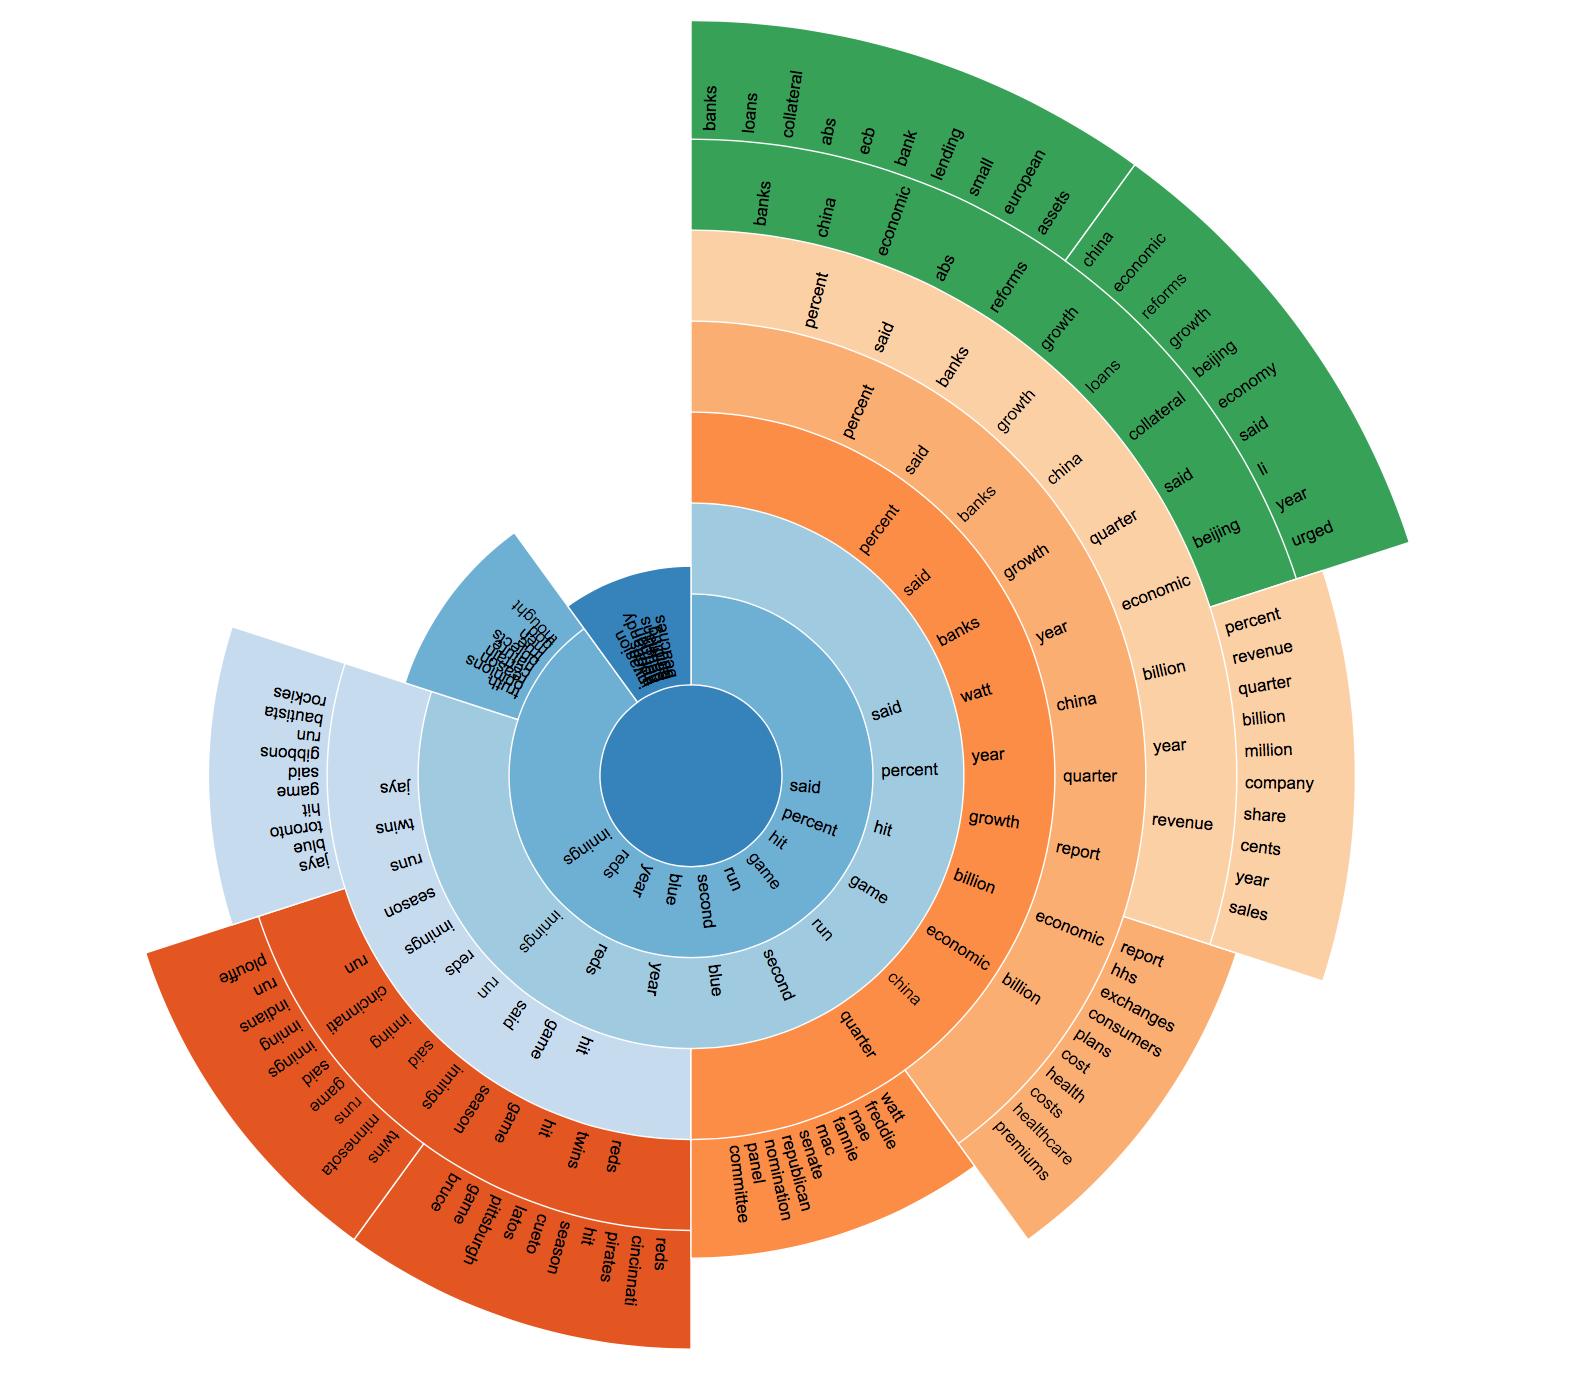
\includegraphics[width=.48\textwidth]{img}
	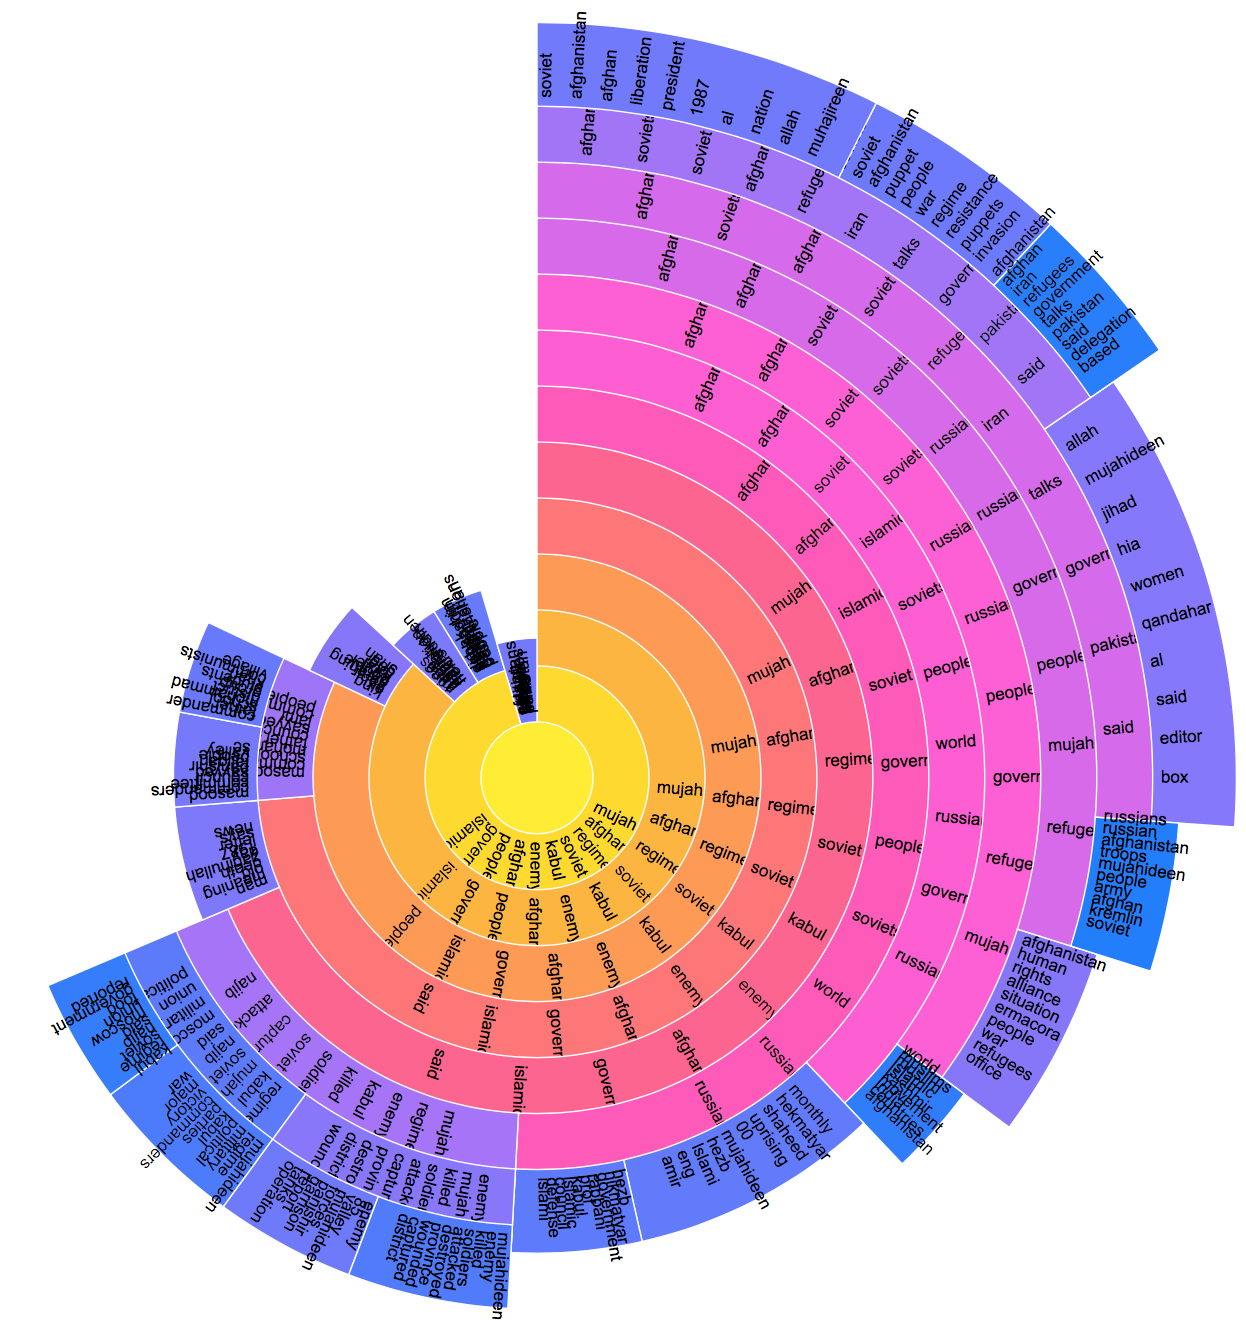
\includegraphics[width=.48\textwidth]{img2}
	\caption{Left: Visualization of hierarchical topics in standard NMF; Right: Visualization of hierarchical topics in  SSNMF; }
\end{figure}
I use the d3.js Sunburst implementation to visualize the hierarchical topic model. Arcs at the same level represent discrete topics. A topic on an inner layer that encompasses multiple outer topics represent a super-topic. For example, in Figure 3, the two outer green topics that represent European banking and Chinese banking representatively (with top words$$ \{\text{banks, loans, collateral, abs, ecb bank, lending, small, european, asset}\} $$and $$\{\text{china, economic, reforms, growth, beijing, economy, said, li, year, urged}\}) $$merge into the inner super topic with top words$$ \{\text{banks, china, economic, abs, reforms, growth, loans, collateral, said, beijing}\}.$$

The visualization is responsive, dynamic and available at \\ \texttt{http://www1.cmc.edu/pages/faculty/BHunter/ziv.html}. The Javascript code uses to generate these sunbursts can be found in the \textbf{Javascript Sunburst} section of the Appendix.

Next, I extended this visualization to the Semi-Supervised domain using the Afghan Dataset. Here each document has associated with it a class $C\in \{1,\cdots,k\}$ which in this case $k=3$. Recall that the matrix $B \in \mathbb{R}^{k \times r}$ in the semi-supervised NMF model is multiplied by $S$ to obtain an approximation for $Y$, the label matrix. Thus the $i,j$th entry of $B$ can be interpreted in the weighted importance of topic $i$ in predicting class $j$. Thus I sum over the columns of $B$ to capture how important topic $i$ is predicting classes in general. After normalizing, we get a color value $c_i$ for topic $i$, such that
$$c_i = \sum_j B_{i,j} /  \sum_{i,j} B_{i,j}$$
where $c_i=1$ corresponds to yellow and $c_i=0$ corresponds to blue (see Figure 3 right)
\begin{figure}
	\centering
	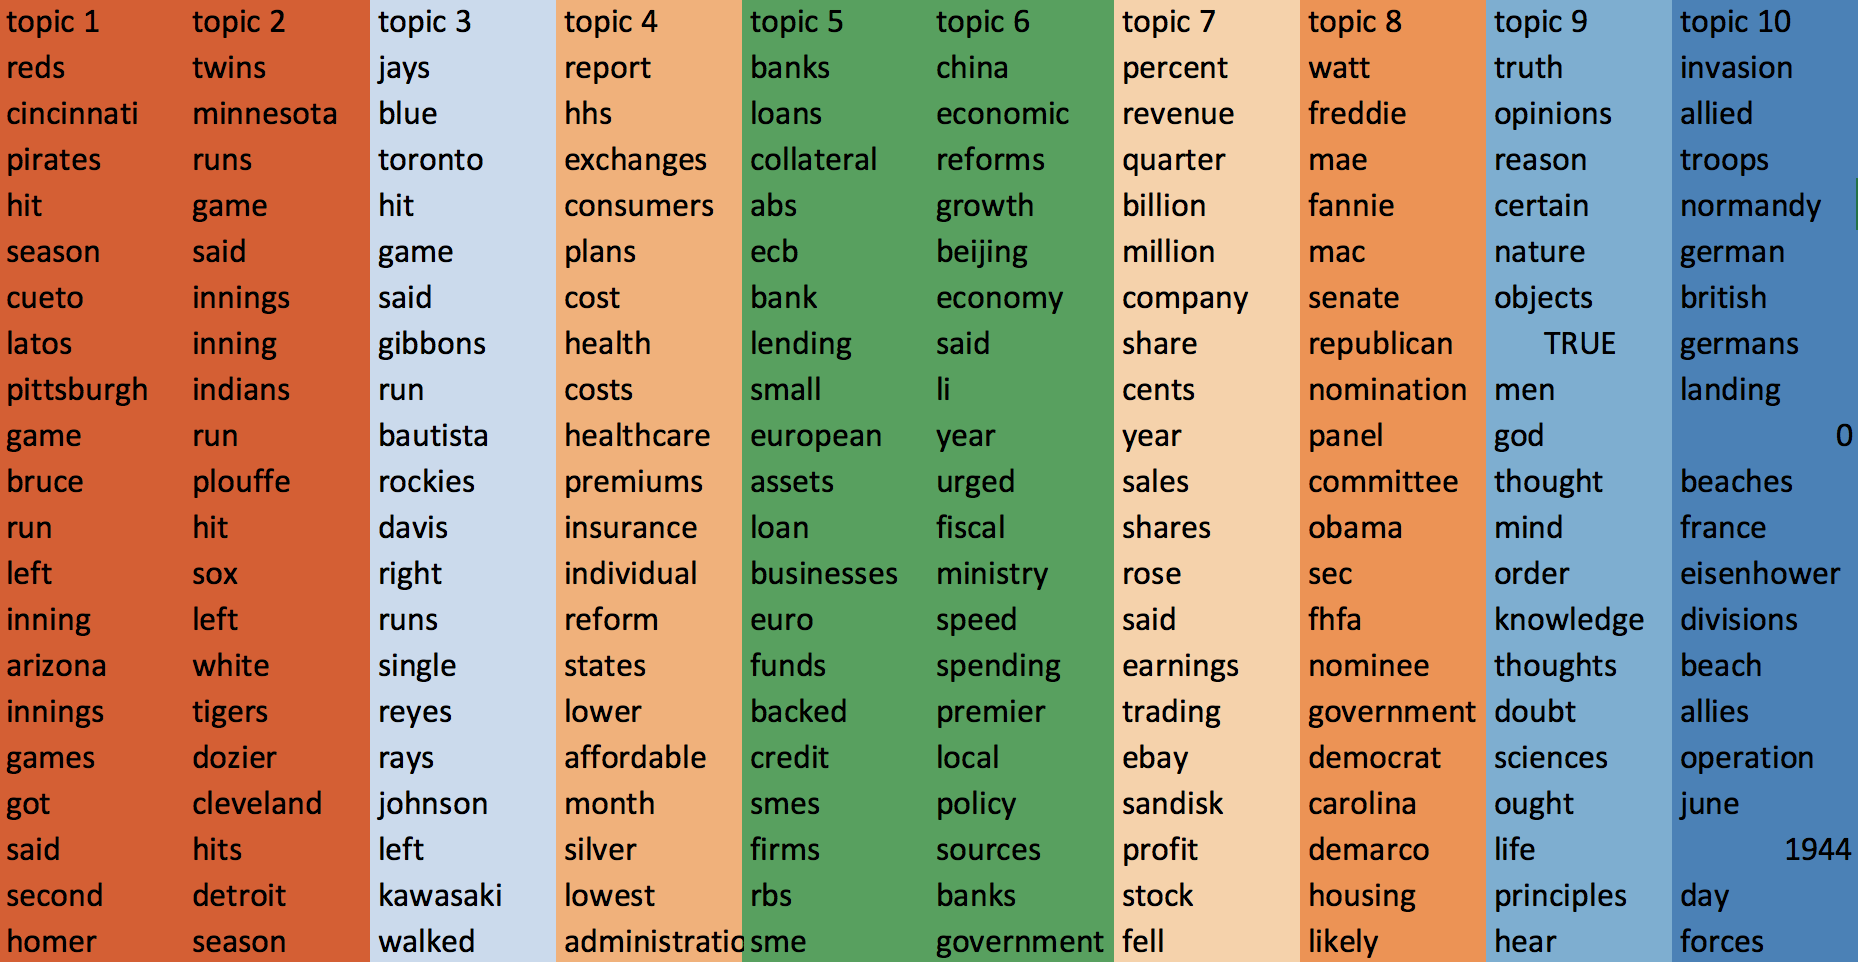
\includegraphics[width=7in]{topic}
	\caption{Topics used in hierarchical topic model}
\end{figure}
\end{chapter}

\section{Deep Models}
\subsection{Motivation}
We next explore the importance of extending the notion of hierarchy from the previous chapter to deep models. This exploration is motivated by the fact that a hierachical organization of information tends to outperform flat schemas in their plasticity and ability to recognize high level concepts.  

Suppose we are trying to learn the function $f$ with $n$ parameters $f(x_1,x_2,\cdots,x_n)$ with a neural network. As shown in Figure \ref{poggio}, the network can either be shallow (left) or deep (right). \begin{figure}
	\label{poggio}
	\centering
	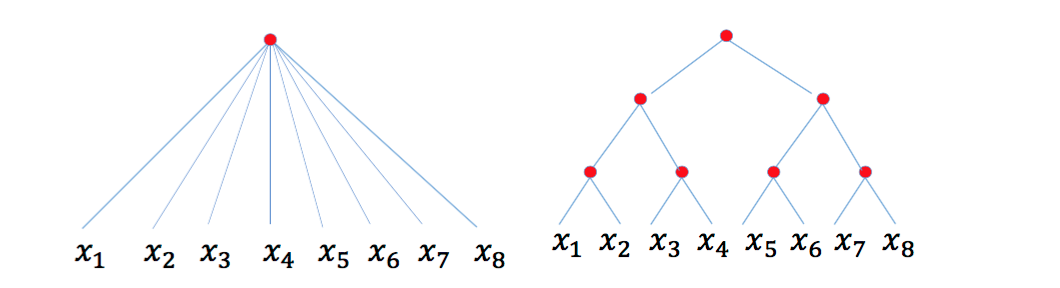
\includegraphics[width=7in]{poggio}
	\caption{A shallow versus deep neural network. The number of parameters a shallow network estimates is exponential in the number of inputs, whereas the number of parameters a deep model estimates is linear in the number of inputs. Image adapted from \cite{mhaskar2016learning}.}
\end{figure}
Both of these networks are \emph{universal}, which is to say that they can both approximate $f$ arbitrarily well. However deep networks with compositional structure -- such that a function specifically of the form $f(x_1, \cdots, x_n) = g_1(g_2\cdots (g_j(g_{i1}(x1,x_2),h_{i2}(x_3,x_4)),\cdots ))$ is learned -- yields the same level of accuracy, while having a substantially smaller number of parameters to estimate, VC-dimension, and fat-shattering dimension \cite{mhaskar2016learning}. Expounding on these ideas, Mhaskar et al. argue that the ``basic properties of scalability and shift invariance in many natural signals such as images and text require compositional algorithms that can be well approximated by \emph{Deep} Convolutional Networks.'' \cite{mhaskar2016learning}
\subsection{A Deep NNMF Model}
Semi-Supervised NNMF as discussed above can be thought of as representing $A$ in a low dimensional representation as $S$. In this framework, $A$ is the function that maps the low dimensional representation to the original high dimensional representation. However, as the data becomes increasingly complex, it may have many hierarchy of attributes, each of which requires its own mappings. With the motivation in mind, Trigeorgis et al put forward the notion of a Demi-Semi NNMF \cite{trigeorgis2014deep}.
$$X \approx A_1A_2 \cdots A_m S_m$$
This representation of the data can be achieved by recursively factorizing the low-dimensional representation at each level \cite{trigeorgis2014deep}.
\begin{align*}
S_{m-1} = A_mS_m\\
\vdots \\
S_2  \approx A_3 \cdots A_m  S_m\\
S_1  \approx A_2 \cdots A_m  S_m
\end{align*}
By recursively factoring, the deep NNMF model learns a hierarchical structure of features such that each level corresponds to a particular attribute of the underlying data (see Figure \ref{deepNNMF}). 
\begin{figure}
	\label{deepNNMF}
	\centering
	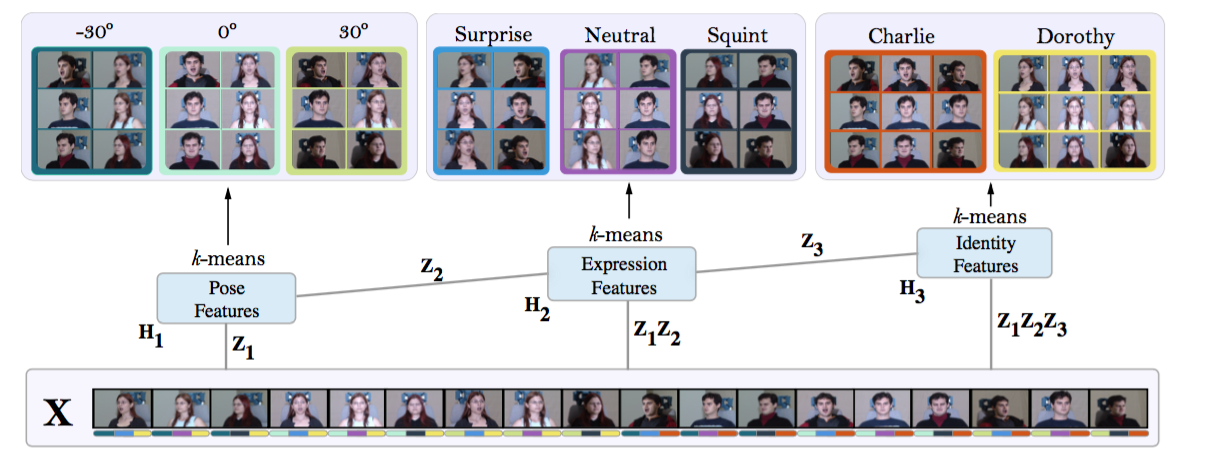
\includegraphics[width=7in]{deep}
	\caption{Recursive factoring results in a hierarchy of attributes. Image adapted from  \cite{trigeorgis2014deep}.}
\end{figure}


\subsection{Deep Neural Models}
	The formulation of recursive matrix factorization above invites a comparison with Deep Neural Networks. As discussed in Chapter \ref{NN}, a neural network can be thought of as a series of matrix multiplications, with a elementwise nonlinear function application between each matrix multiplication. Thus Trigeorgis et al's recursive formulation is in fact more than halfway to a deep neural network. Flenner and Hunter formalize this intuition with their so called Deep NNMF \cite{deepNonNeg}. In particular, they take advantage of the fact that the most well used non-linearity function in Deep Neural Networks is the rectifyer activation function $g(z)=\max(0,z)$. This is relevant because this function is equivalent to NNMF's restriction of positive entries in the learned matrices.  
\begin{chapter}{Discussion}
	In this thesis, I explored a suite of non-negative matrix factorization algorithms. In recent years, NNMF has emerged as a powerful new way to perform dimensionality reduction, topic modelling, and data visualization, among others. Because of its broad applications, there are many variants of traditional NNMF that have made their way to the main stream, such as graph regularized, supervised, hiearchical, deep, etc. Many of these variants explore the same functionality that the visual perceptual literature is interested in.  A central tenant of this thesis was to use many of the NNMF variants that relate to the cognitive underpinnings to underscore the plasticity and power of this suite of algorithms. It is important to note that I am not directly claiming that for image recognition, our brain actually implements non-negative matrix factorization. In that sense, the analogy fails. However, the regularizers for manifold and supervised learning, coupled with the arbitrary amounts of complexity that can introduced via hierarchy and deep NNMF suggest that key cognitive elements of the human understanding machine can be formalized as algorithmic models. 
	
	There are several next steps for this inquiry, along different axes. The first is applying the canonical visualization techniques of NNMF to deep (neural) models. As deep models such as neural networks become more pervasive in industry and the academy, gaining windows to understand mechanism becomes increasingly important. In the future, I hope deep models can adopt the suite of visualization and interpretation tactics that the NNMF literature uses to gain understanding about their inner workings. 
	
	Another domain for exploration is the space of hierarchy. In this thesis, I explored a bottom-up, agglomerative hierarchical clustering algorithm. While this technique yields reasonable results, it is unclear if this method is optimal. I also touch on the idea of a deep implementation. While this was not the central focus of this document, I think those ideas are on the cutting edge of novel NNMF discoveries, and warrants conclusion. In the future, I hope advances in the technical understanding of the hierarchical nature of human perception will lead to an hierarchical clustering algorithm that can be implemented in this domain.
	
	A final area of inquiry that extends the ideas of this thesis would be the formalization of the Manifold NNMF put forward in Chapter \ref{mNNMF}, with an added hierarchical component. By mirroring the architecture necessary to learn continuous manifolds, coupled with the representation complexity achieved via a hierarchy of models, the class of representations that can be described will increase. 
	\end{chapter}
\section*{Acknowledgments}
I would like the thank the Pomona College Math Department for their tireless support and guidance.  I would like to thank Professor Blake Hunter, Leo Selker, Dima Smirnov, Professor Shlomi Sher, Neo Mohsenvand for invaluable comments, ideas, inspiration and discussion. 
\newpage
\section*{Appendix}
\subsection*{Datasets}
For this thesis, I used two datasets to generate all the models, both of which are a collection of documents. 
\subsubsection*{20 News Groups}
This canonical NLP dataset consists of approximately 20,000 newsgroup documents across 20 different newsgroups. It was originally collected by Ken Lang and has been by NLP researchers in a variety of applicaitons \cite{20news}. For the purposes of this thesis, I used a small subset of the full data set, with 98 documents. 

Because 20 News Groups is so well established in the literature, I use it as a canned dataset to verify that the algorithms I implemented are indeed doing something reasonable. 
\subsubsection*{Afghan Mujahideen}
To accompany the canned dataset, I used a more interesting and culturally significant source of data. This is a corpus of documents published by ``Afghan mujahideen forces fighting Soviet and Afghan communists forces between 1980 and 1992'' curated by NYU Abu Dhabi Sociologist Daniel Karell.
\subsection*{Graph Regularized NNMF}
\begin{lstlisting}
from sklearn.feature_extraction.text import TfidfVectorizer, CountVectorizer
from sklearn.decomposition import NMF
from sklearn.datasets import fetch_20newsgroups
from sklearn.metrics.pairwise import cosine_similarity as cosine
from scipy.sparse.csgraph import connected_components
import itertools
import json
import numpy as np
import glob
local_data = []
philes =  glob.glob("/Users/ziv/GDrive/school/math-thesis/nmf-imp/data/*.txt")
for phile in philes:
	with open(phile, 'r') as myfile:
		data=myfile.read().replace('\n', '')
		local_data.append(unicode(data, errors='ignore'))
tfidf_vectorizer = TfidfVectorizer(max_df=0.95, min_df=2, #max_features=n_features,
stop_words='english')

tfidf = tfidf_vectorizer.fit_transform(local_data)
tfidf_feature_names = tfidf_vectorizer.get_feature_names()

def generate_graphs(X,p):
	W_raw = np.zeros((X.shape[1],X.shape[1]))
	for i in range(0,X.shape[0]):
		for j in range(0,X.shape[0]):
			W_raw[i,j] = np.dot(X[i,], t(X[j,]))[0,0]
	s = W_raw.flatten()
	thresh = np.percentile(s,p)
	W = (W_raw > thresh).astype(int)
	D = np.zeros((X.shape[1],X.shape[1]))
	for i in range(0,X.shape[0]):
		D[i,i] = sum(W[i,])
	return W,D
	
def grnmf(X,k,lam,p,u0=None,v0=None):
	W,D = generate_graphs(X,p)
	if u0==None: 
		u = np.random.rand(X.shape[0],k)
	else:
		u = u0
	if v0==None:
		v = np.random.rand(X.shape[1],k)
	else:
		v = v0
	i = 0    
	while i < 1000:
		u = u = np.multiply(u,((X*v)/ np.dot(np.dot(u,t(v)),v)))
		v = np.multiply(v , ((np.dot(t(X),u) + 0.2*np.dot(W,v))/ (np.dot(np.dot(v,t(u)),u) + .2*np.dot(D,v))))
		i +=1
		if i % 5 ==0:
		print str(i) + "/1000 iterations complete"
	return u,v
	
def t(x):
	return np.transpose(x)
	
u,v = grnmf(X,k=10,lam=0.2,p=90)
\end{lstlisting}
\subsection*{Semi-Supervised NNMF}
\begin{lstlisting}
get_ipython().magic(u'matplotlib inline')
import numpy as np
import matplotlib.pylab as plt
import random
import glob
from sklearn.feature_extraction.text import TfidfVectorizer, CountVectorizer

def ssnmf(X,L,Y,lamb,r,k,A0=None,S0=None):
	if A0==None: 
		A = np.random.rand(X.shape[0],r)
	else:
		A = A0
	if S0==None:
		S = np.random.rand(r,X.shape[1])
	else:
		S = S0
	B = np.random.rand(k,r)
	i = 0  
	while i < 100:
		A = A * (np.dot(X,t(S))/ np.dot(np.dot(A,S),t(S)))
		B = B * (np.dot((L * Y), t(S)))/np.dot((L * np.dot(B,S)), t(S))
		S = S * (np.dot(t(A),X) + lamb*np.dot(t(B),L*Y))/(np.dot(t(A),np.dot(A,S)) + lamb*np.dot(t(B),L*np.dot(B,S)))
		i +=1
		if i%20 == 0:
		print i
	return A,S,B
def t(x):
	return np.transpose(x)
\end{lstlisting}
\subsection*{Building a hierarchy}
\begin{lstlisting}
local_data = []
philes =  glob.glob("/Users/ziv/GDrive/school/math-thesis/nmf-imp/txt_data_bypage/*.txt")
for phile in philes:
with open(phile, 'r') as myfile:
data=myfile.read().replace('\n', '')
local_data.append(unicode(data, errors='ignore'))
tfidf_vectorizer = TfidfVectorizer(max_df=0.95, min_df=2, #max_features=n_features,
stop_words='english')

tfidf = tfidf_vectorizer.fit_transform(local_data)
tfidf_feature_names = tfidf_vectorizer.get_feature_names()
nmf = NMF(n_components=n_topics).fit(tfidf)
H = nmf.components_
W = nmf.fit_transform(tfidf)
weights = (5000/W.sum())*W.sum(axis=0)

def build_wgraph(alpha=2):
	if alpha != 2:
		return [[int(cosine(H[i],H[j])[0][0] > alpha) for i in range(0, len(H))] for j in range(0, len(H))]
	else:
		return [[cosine(H[i],H[j])[0][0] for i in range(0, len(H))] for j in range(0, len(H))]
def thresh_vals(numbin):
	binz = []
	w = build_wgraph(2)
	chain = itertools.chain(*w)
	s =sorted(list(chain))
	val = n_topics*n_topics/numbin
	for i,v in enumerate(s):
		if i%val ==0: binz.append(v)
	return binz
	}    
}

def array_distance(A,B):
	count = 0
	for i,x in enumerate(A):
		if x == B[i]:
			count+=1
	return len(A)-count

def greedy_TV_build(to_consume,bins):
	if len(to_consume)>1:
		a = to_consume[0]
		b = to_consume[1]
		ccA = connected_components(build_wgraph(a))[1]
		ccB = connected_components(build_wgraph(b))[1]
		if not np.array_equal(ccA, ccB):
			distance = array_distance(ccA,ccB)
			if distance > 8:
				new_tv = [a + i*(b-a)/bins for i in range(0,bins)]
				return new_tv + greedy_TV_build( to_consume[1:], bins)
			else:
				return [a] + greedy_TV_build(to_consume[1:], bins)
		else:
			return greedy_TV_build(to_consume[1:], bins)
	elif len(to_consume) == 1:
		return to_consume
	else:
	return []
def populateTree(row_level, valid_community):
	if row_level > size-2 :
		return []
	else:
		children = []
		parent_community = connected_components(build_wgraph(tv[row_level]))[1]
		child_community = connected_components(build_wgraph(tv[row_level+1]))[1]
		unique_communities = list(set(parent_community)) 
		for unique_community in unique_communities:
			if valid_community == unique_community:
				indices = [i for i, x in enumerate(parent_community) if x == unique_community] #[8,9]
				seen_communities = []
			for i in indices: #8 and 9
				if child_community[i] in seen_communities:
					filter(lambda x: x['community'] == str(child_community[i]), children)[0]['indices'].append(i)
				else:
					community_to_find = child_community[i]
					grow_my_children = populateTree(row_level+1, community_to_find)
					if grow_my_children:
						name = ""
						children.append({"community":str(child_community[i]),"indices":[i],"name" : name , "children":grow_my_children, "hasChildren": True})
					else:
						name = " ".join([tfidf_feature_names[j] for j in nmf.components_[i].argsort()[:-n_top_words - 1:-1]])
						children.append({"community":str(child_community[i]),"indices":[i],"size":weights[i],"name":name, "hasChildren": False})
					seen_communities.append(child_community[i])
			if len(children) == 1:
				try: 
					return children[0]['children']
				except:
					return []
			else:
				return children

def recursiveNaming(tree):
	i = tree['indices']
	base = nmf.components_[i[0]]
	if len(i) > 1:
		for ind in i[1:]:
			base = np.add(nmf.components_[ind], base)
	tree['name'] = " ".join([tfidf_feature_names[j] for j in base.argsort()[:-n_top_words - 1:-1]])
	if tree['hasChildren']:
	for child in tree['children']:
		recursiveNaming(child)
		
tv = greedy_TV_build(thresh_vals(100),2)
size = len(tv)
flare = {"name" : "" , "children" : populateTree(0, 0)}
for child in flare['children']:
recursiveNaming(child)
with open('demo.json', 'w') as outfile:
json.dump(flare, outfile)
\end{lstlisting}
\subsection*{Javascript Sunburst}
\begin{lstlisting}
<script>

var width = 1260,
height = 1100,
radius = Math.min(width, height) / 2.1;

var x = d3.scale.linear()
.range([0, 2 * Math.PI]);

var y = d3.scale.linear()
.range([0, radius]);

var color = d3.scale.category20c();

var svg = d3.select("body").append("svg")
.attr("width", width)
.attr("height", height)
.append("g")
.attr("transform", "translate(" + width / 2 + "," + (height / 2 + 10) + ")");

var partition = d3.layout.partition()
.value(function(d) { return d.size; });

var arc = d3.svg.arc()
.startAngle(function(d) { return Math.max(0, Math.min(2 * Math.PI, x(d.x))); })
.endAngle(function(d) { return Math.max(0, Math.min(2 * Math.PI, x(d.x + d.dx))); })
.innerRadius(function(d) { return Math.max(0, y(d.y)); })
.outerRadius(function(d) { return Math.max(0, 20+y(d.y + d.dy)); });

d3.json("20news.json", function(error, root) {
var g = svg.selectAll("g")
.data(partition.nodes(root))
.enter().append("g");

var path = g.append("path")
.attr("d", arc)
.style("fill", function(d) { return color((d.children ? d : d.parent).name); })
.on("click", click);

var text = []
for (i = 0; i < 10; i++) { 
var localText = g.append("text")
.attr("transform", function(d) { 
var theta = Math.max(0, Math.min(2 * Math.PI, x(d.x + d.dx))) - Math.max(0, Math.min(2 * Math.PI, x(d.x))) 
var scale_factor = theta * Math.sqrt(Math.max(0, y(d.y + d.dy)))
var offset = 2.4*scale_factor / 10 
return "rotate(" + computeTextRotation(d,offset*i,scale_factor ) + ")"; 
})
.attr("x", function(d) { return y(d.y); })
.attr("dx", "6") // margin
.attr("dy", ".35em") // vertical-align
.attr("class", "topicText".concat(i))
.text(function(d) {
return d.name.split(" ")[i]
});
text.push(localText)
}

function click(d) {
// fade out all text elements
for (i = 0; i < 10; i++) { 
text[i].transition().attr("opacity", 0);
}

path.transition()
.duration(750)
.attrTween("d", arcTween(d))
.each("end", function(e, i) {
if (e.x >= d.x && e.x < (d.x + d.dx)) {
// get a selection of the associated text element
for (j = 0; j < 10; j++) { 
var arcText = d3.select(this.parentNode).select(".topicText".concat(j));
console.log(arcText);
// fade in the text element and recalculate positions
arcText.transition().duration(750)
.attr("opacity", 1)
.attr("transform", function() { 
var theta = Math.max(0, Math.min(2 * Math.PI, x(e.x + e.dx))) - Math.max(0, Math.min(2 * Math.PI, x(e.x))) 
var scale_factor = theta * Math.sqrt(Math.max(0, y(e.y + e.dy)))
var offset = 2.4*scale_factor / 10 
return "rotate(" + computeTextRotation(e,j*offset,scale_factor ) + ")" 
})
.attr("x", function(d) { return y(d.y); });
}
}
});
}
});

d3.select(self.frameElement).style("height", height + "px");

// Interpolate the scales!
function arcTween(d) {
var xd = d3.interpolate(x.domain(), [d.x, d.x + d.dx]),
yd = d3.interpolate(y.domain(), [d.y, 1]),
yr = d3.interpolate(y.range(), [d.y ? 20 : 0, radius]);
return function(d, i) {
return i
? function(t) { return arc(d); }
: function(t) { x.domain(xd(t)); y.domain(yd(t)).range(yr(t)); return arc(d); };
};
}

function computeTextRotation(d,inc, sf) {
return inc-sf-2+(x(d.x + d.dx / 2) - Math.PI / 2) / Math.PI * 180;
}

function computeTextRotationUpdate(d) {
return (x(d.x + d.dx / 2) - Math.PI / 2) / Math.PI * 180;
}

</script>
\end{lstlisting}
\bibliographystyle{plain}

\bibliography{myBib}
\end{document}